% Path A paper: draft. All results come from paper/generated/ (scripts/paper_assets.py).
\documentclass[5p,times]{elsarticle}

\usepackage[T1]{fontenc}
\usepackage{amsmath,amssymb}
\usepackage{booktabs}
\usepackage{graphicx}
\usepackage{xcolor}
\usepackage{tikz}
\usetikzlibrary{positioning,calc,arrows.meta}
\usepackage[hidelinks]{hyperref}

\definecolor{lblue}{HTML}{2A78D6}
\definecolor{lorange}{HTML}{EB6834}
% visible markers for unfinished parts of the draft
\newcommand{\pending}[1]{\textcolor{red}{[PENDING: #1]}}
\newcommand{\verify}[1]{\textcolor{red}{[VERIFY: #1]}}

% generated by scripts/paper_assets.py from results/analysis/pathA -- do not edit
\providecommand\res[1]{\csname res@#1\endcsname}
\expandafter\def\csname res@H1-CEC2022-ci\endcsname{[0.434, 0.489]}
\expandafter\def\csname res@H1-CEC2022-i1-amed\endcsname{2.43{\times}10^{-7}}
\expandafter\def\csname res@H1-CEC2022-i1-cmed\endcsname{1.59{\times}10^{-7}}
\expandafter\def\csname res@H1-CEC2022-i1-w\endcsname{0.36}
\expandafter\def\csname res@H1-CEC2022-i10-amed\endcsname{100.4}
\expandafter\def\csname res@H1-CEC2022-i10-cmed\endcsname{100.4}
\expandafter\def\csname res@H1-CEC2022-i10-w\endcsname{0.52}
\expandafter\def\csname res@H1-CEC2022-i11-amed\endcsname{300}
\expandafter\def\csname res@H1-CEC2022-i11-cmed\endcsname{300}
\expandafter\def\csname res@H1-CEC2022-i11-w\endcsname{0.54}
\expandafter\def\csname res@H1-CEC2022-i12-amed\endcsname{240.1}
\expandafter\def\csname res@H1-CEC2022-i12-cmed\endcsname{240.8}
\expandafter\def\csname res@H1-CEC2022-i12-w\endcsname{0.49}
\expandafter\def\csname res@H1-CEC2022-i2-amed\endcsname{44.9}
\expandafter\def\csname res@H1-CEC2022-i2-cmed\endcsname{49.08}
\expandafter\def\csname res@H1-CEC2022-i2-w\endcsname{0.43}
\expandafter\def\csname res@H1-CEC2022-i3-amed\endcsname{1.63{\times}10^{-5}}
\expandafter\def\csname res@H1-CEC2022-i3-cmed\endcsname{4.39{\times}10^{-6}}
\expandafter\def\csname res@H1-CEC2022-i3-w\endcsname{0.21}
\expandafter\def\csname res@H1-CEC2022-i4-amed\endcsname{37.31}
\expandafter\def\csname res@H1-CEC2022-i4-cmed\endcsname{33.83}
\expandafter\def\csname res@H1-CEC2022-i4-w\endcsname{0.38}
\expandafter\def\csname res@H1-CEC2022-i5-amed\endcsname{17.67}
\expandafter\def\csname res@H1-CEC2022-i5-cmed\endcsname{17.04}
\expandafter\def\csname res@H1-CEC2022-i5-w\endcsname{0.54}
\expandafter\def\csname res@H1-CEC2022-i6-amed\endcsname{20.02}
\expandafter\def\csname res@H1-CEC2022-i6-cmed\endcsname{17.65}
\expandafter\def\csname res@H1-CEC2022-i6-w\endcsname{0.51}
\expandafter\def\csname res@H1-CEC2022-i7-amed\endcsname{30.1}
\expandafter\def\csname res@H1-CEC2022-i7-cmed\endcsname{29.92}
\expandafter\def\csname res@H1-CEC2022-i7-w\endcsname{0.47}
\expandafter\def\csname res@H1-CEC2022-i8-amed\endcsname{20.96}
\expandafter\def\csname res@H1-CEC2022-i8-cmed\endcsname{21.01}
\expandafter\def\csname res@H1-CEC2022-i8-w\endcsname{0.46}
\expandafter\def\csname res@H1-CEC2022-i9-amed\endcsname{180.8}
\expandafter\def\csname res@H1-CEC2022-i9-cmed\endcsname{180.8}
\expandafter\def\csname res@H1-CEC2022-i9-w\endcsname{0.62}
\expandafter\def\csname res@H1-CEC2022-n\endcsname{12}
\expandafter\def\csname res@H1-CEC2022-rel\endcsname{-4.3{\times}10^{-4}}
\expandafter\def\csname res@H1-CEC2022-relmax\endcsname{2.4{\times}10^{0}}
\expandafter\def\csname res@H1-CEC2022-siga\endcsname{0}
\expandafter\def\csname res@H1-CEC2022-sigc\endcsname{1}
\expandafter\def\csname res@H1-CEC2022-verdict\endcsname{comparator superior}
\expandafter\def\csname res@H1-CEC2022-wbar\endcsname{0.461}
\expandafter\def\csname res@H1-FIR-ci\endcsname{[0.409, 0.476]}
\expandafter\def\csname res@H1-FIR-i1-amed\endcsname{5.17{\times}10^{-3}}
\expandafter\def\csname res@H1-FIR-i1-cmed\endcsname{4.81{\times}10^{-3}}
\expandafter\def\csname res@H1-FIR-i1-w\endcsname{0.28}
\expandafter\def\csname res@H1-FIR-i2-amed\endcsname{0.02158}
\expandafter\def\csname res@H1-FIR-i2-cmed\endcsname{0.02137}
\expandafter\def\csname res@H1-FIR-i2-w\endcsname{0.47}
\expandafter\def\csname res@H1-FIR-i3-amed\endcsname{5.09{\times}10^{-3}}
\expandafter\def\csname res@H1-FIR-i3-cmed\endcsname{4.82{\times}10^{-3}}
\expandafter\def\csname res@H1-FIR-i3-w\endcsname{0.39}
\expandafter\def\csname res@H1-FIR-i4-amed\endcsname{0.02151}
\expandafter\def\csname res@H1-FIR-i4-cmed\endcsname{0.02124}
\expandafter\def\csname res@H1-FIR-i4-w\endcsname{0.51}
\expandafter\def\csname res@H1-FIR-i5-amed\endcsname{1.74{\times}10^{-3}}
\expandafter\def\csname res@H1-FIR-i5-cmed\endcsname{1.41{\times}10^{-3}}
\expandafter\def\csname res@H1-FIR-i5-w\endcsname{0.36}
\expandafter\def\csname res@H1-FIR-i6-amed\endcsname{8.34{\times}10^{-3}}
\expandafter\def\csname res@H1-FIR-i6-cmed\endcsname{6.77{\times}10^{-3}}
\expandafter\def\csname res@H1-FIR-i6-w\endcsname{0.47}
\expandafter\def\csname res@H1-FIR-i7-amed\endcsname{1.32{\times}10^{-3}}
\expandafter\def\csname res@H1-FIR-i7-cmed\endcsname{1.60{\times}10^{-3}}
\expandafter\def\csname res@H1-FIR-i7-w\endcsname{0.52}
\expandafter\def\csname res@H1-FIR-i8-amed\endcsname{3.69{\times}10^{-3}}
\expandafter\def\csname res@H1-FIR-i8-cmed\endcsname{3.81{\times}10^{-3}}
\expandafter\def\csname res@H1-FIR-i8-w\endcsname{0.54}
\expandafter\def\csname res@H1-FIR-n\endcsname{8}
\expandafter\def\csname res@H1-FIR-rel\endcsname{-1.1{\times}10^{-2}}
\expandafter\def\csname res@H1-FIR-relmax\endcsname{1.4{\times}10^{-1}}
\expandafter\def\csname res@H1-FIR-siga\endcsname{0}
\expandafter\def\csname res@H1-FIR-sigc\endcsname{1}
\expandafter\def\csname res@H1-FIR-verdict\endcsname{comparator superior}
\expandafter\def\csname res@H1-FIR-wbar\endcsname{0.443}
\expandafter\def\csname res@H2a-CEC2022-ci\endcsname{[0.495, 0.573]}
\expandafter\def\csname res@H2a-CEC2022-i1-amed\endcsname{6.25{\times}10^{-13}}
\expandafter\def\csname res@H2a-CEC2022-i1-cmed\endcsname{3.98{\times}10^{-13}}
\expandafter\def\csname res@H2a-CEC2022-i1-w\endcsname{0.44}
\expandafter\def\csname res@H2a-CEC2022-i10-amed\endcsname{137.2}
\expandafter\def\csname res@H2a-CEC2022-i10-cmed\endcsname{101.5}
\expandafter\def\csname res@H2a-CEC2022-i10-w\endcsname{0.42}
\expandafter\def\csname res@H2a-CEC2022-i11-amed\endcsname{300}
\expandafter\def\csname res@H2a-CEC2022-i11-cmed\endcsname{300}
\expandafter\def\csname res@H2a-CEC2022-i11-w\endcsname{0.59}
\expandafter\def\csname res@H2a-CEC2022-i12-amed\endcsname{251.5}
\expandafter\def\csname res@H2a-CEC2022-i12-cmed\endcsname{251.7}
\expandafter\def\csname res@H2a-CEC2022-i12-w\endcsname{0.49}
\expandafter\def\csname res@H2a-CEC2022-i2-amed\endcsname{49.08}
\expandafter\def\csname res@H2a-CEC2022-i2-cmed\endcsname{46.99}
\expandafter\def\csname res@H2a-CEC2022-i2-w\endcsname{0.57}
\expandafter\def\csname res@H2a-CEC2022-i3-amed\endcsname{0.5583}
\expandafter\def\csname res@H2a-CEC2022-i3-cmed\endcsname{0.5669}
\expandafter\def\csname res@H2a-CEC2022-i3-w\endcsname{0.60}
\expandafter\def\csname res@H2a-CEC2022-i4-amed\endcsname{38.8}
\expandafter\def\csname res@H2a-CEC2022-i4-cmed\endcsname{45.77}
\expandafter\def\csname res@H2a-CEC2022-i4-w\endcsname{0.62}
\expandafter\def\csname res@H2a-CEC2022-i5-amed\endcsname{417.6}
\expandafter\def\csname res@H2a-CEC2022-i5-cmed\endcsname{330.8}
\expandafter\def\csname res@H2a-CEC2022-i5-w\endcsname{0.40}
\expandafter\def\csname res@H2a-CEC2022-i6-amed\endcsname{39.17}
\expandafter\def\csname res@H2a-CEC2022-i6-cmed\endcsname{45.1}
\expandafter\def\csname res@H2a-CEC2022-i6-w\endcsname{0.62}
\expandafter\def\csname res@H2a-CEC2022-i7-amed\endcsname{57.09}
\expandafter\def\csname res@H2a-CEC2022-i7-cmed\endcsname{56.02}
\expandafter\def\csname res@H2a-CEC2022-i7-w\endcsname{0.56}
\expandafter\def\csname res@H2a-CEC2022-i8-amed\endcsname{22.77}
\expandafter\def\csname res@H2a-CEC2022-i8-cmed\endcsname{22.92}
\expandafter\def\csname res@H2a-CEC2022-i8-w\endcsname{0.42}
\expandafter\def\csname res@H2a-CEC2022-i9-amed\endcsname{180.8}
\expandafter\def\csname res@H2a-CEC2022-i9-cmed\endcsname{180.8}
\expandafter\def\csname res@H2a-CEC2022-i9-w\endcsname{0.68}
\expandafter\def\csname res@H2a-CEC2022-n\endcsname{12}
\expandafter\def\csname res@H2a-CEC2022-rel\endcsname{6.3{\times}10^{-12}}
\expandafter\def\csname res@H2a-CEC2022-relmax\endcsname{1.0{\times}10^{0}}
\expandafter\def\csname res@H2a-CEC2022-siga\endcsname{0}
\expandafter\def\csname res@H2a-CEC2022-sigc\endcsname{0}
\expandafter\def\csname res@H2a-CEC2022-verdict\endcsname{inconclusive}
\expandafter\def\csname res@H2a-CEC2022-wbar\endcsname{0.534}
\expandafter\def\csname res@H2a-FIR-ci\endcsname{[0.527, 0.623]}
\expandafter\def\csname res@H2a-FIR-i1-amed\endcsname{4.85{\times}10^{-3}}
\expandafter\def\csname res@H2a-FIR-i1-cmed\endcsname{4.92{\times}10^{-3}}
\expandafter\def\csname res@H2a-FIR-i1-w\endcsname{0.56}
\expandafter\def\csname res@H2a-FIR-i2-amed\endcsname{0.02128}
\expandafter\def\csname res@H2a-FIR-i2-cmed\endcsname{0.02121}
\expandafter\def\csname res@H2a-FIR-i2-w\endcsname{0.46}
\expandafter\def\csname res@H2a-FIR-i3-amed\endcsname{4.81{\times}10^{-3}}
\expandafter\def\csname res@H2a-FIR-i3-cmed\endcsname{5.13{\times}10^{-3}}
\expandafter\def\csname res@H2a-FIR-i3-w\endcsname{0.58}
\expandafter\def\csname res@H2a-FIR-i4-amed\endcsname{0.02136}
\expandafter\def\csname res@H2a-FIR-i4-cmed\endcsname{0.022}
\expandafter\def\csname res@H2a-FIR-i4-w\endcsname{0.60}
\expandafter\def\csname res@H2a-FIR-i5-amed\endcsname{1.35{\times}10^{-3}}
\expandafter\def\csname res@H2a-FIR-i5-cmed\endcsname{2.04{\times}10^{-3}}
\expandafter\def\csname res@H2a-FIR-i5-w\endcsname{0.68}
\expandafter\def\csname res@H2a-FIR-i6-amed\endcsname{7.53{\times}10^{-3}}
\expandafter\def\csname res@H2a-FIR-i6-cmed\endcsname{7.29{\times}10^{-3}}
\expandafter\def\csname res@H2a-FIR-i6-w\endcsname{0.52}
\expandafter\def\csname res@H2a-FIR-i7-amed\endcsname{1.66{\times}10^{-3}}
\expandafter\def\csname res@H2a-FIR-i7-cmed\endcsname{1.88{\times}10^{-3}}
\expandafter\def\csname res@H2a-FIR-i7-w\endcsname{0.62}
\expandafter\def\csname res@H2a-FIR-i8-amed\endcsname{3.64{\times}10^{-3}}
\expandafter\def\csname res@H2a-FIR-i8-cmed\endcsname{3.98{\times}10^{-3}}
\expandafter\def\csname res@H2a-FIR-i8-w\endcsname{0.58}
\expandafter\def\csname res@H2a-FIR-n\endcsname{8}
\expandafter\def\csname res@H2a-FIR-rel\endcsname{1.4{\times}10^{-2}}
\expandafter\def\csname res@H2a-FIR-relmax\endcsname{1.6{\times}10^{-1}}
\expandafter\def\csname res@H2a-FIR-siga\endcsname{1}
\expandafter\def\csname res@H2a-FIR-sigc\endcsname{0}
\expandafter\def\csname res@H2a-FIR-verdict\endcsname{anchor superior}
\expandafter\def\csname res@H2a-FIR-wbar\endcsname{0.575}
\expandafter\def\csname res@H2b-CEC2022-ci\endcsname{[0.690, 0.743]}
\expandafter\def\csname res@H2b-CEC2022-i1-amed\endcsname{2.33{\times}10^{-7}}
\expandafter\def\csname res@H2b-CEC2022-i1-cmed\endcsname{6.25{\times}10^{-13}}
\expandafter\def\csname res@H2b-CEC2022-i1-w\endcsname{0.12}
\expandafter\def\csname res@H2b-CEC2022-i10-amed\endcsname{100.4}
\expandafter\def\csname res@H2b-CEC2022-i10-cmed\endcsname{137.2}
\expandafter\def\csname res@H2b-CEC2022-i10-w\endcsname{0.92}
\expandafter\def\csname res@H2b-CEC2022-i11-amed\endcsname{300}
\expandafter\def\csname res@H2b-CEC2022-i11-cmed\endcsname{300}
\expandafter\def\csname res@H2b-CEC2022-i11-w\endcsname{0.18}
\expandafter\def\csname res@H2b-CEC2022-i12-amed\endcsname{241.6}
\expandafter\def\csname res@H2b-CEC2022-i12-cmed\endcsname{251.5}
\expandafter\def\csname res@H2b-CEC2022-i12-w\endcsname{0.92}
\expandafter\def\csname res@H2b-CEC2022-i2-amed\endcsname{49.08}
\expandafter\def\csname res@H2b-CEC2022-i2-cmed\endcsname{49.08}
\expandafter\def\csname res@H2b-CEC2022-i2-w\endcsname{0.36}
\expandafter\def\csname res@H2b-CEC2022-i3-amed\endcsname{4.01{\times}10^{-6}}
\expandafter\def\csname res@H2b-CEC2022-i3-cmed\endcsname{0.5583}
\expandafter\def\csname res@H2b-CEC2022-i3-w\endcsname{1.00}
\expandafter\def\csname res@H2b-CEC2022-i4-amed\endcsname{29.85}
\expandafter\def\csname res@H2b-CEC2022-i4-cmed\endcsname{38.8}
\expandafter\def\csname res@H2b-CEC2022-i4-w\endcsname{0.72}
\expandafter\def\csname res@H2b-CEC2022-i5-amed\endcsname{16.53}
\expandafter\def\csname res@H2b-CEC2022-i5-cmed\endcsname{417.6}
\expandafter\def\csname res@H2b-CEC2022-i5-w\endcsname{1.00}
\expandafter\def\csname res@H2b-CEC2022-i6-amed\endcsname{16.05}
\expandafter\def\csname res@H2b-CEC2022-i6-cmed\endcsname{39.17}
\expandafter\def\csname res@H2b-CEC2022-i6-w\endcsname{0.82}
\expandafter\def\csname res@H2b-CEC2022-i7-amed\endcsname{31.1}
\expandafter\def\csname res@H2b-CEC2022-i7-cmed\endcsname{57.09}
\expandafter\def\csname res@H2b-CEC2022-i7-w\endcsname{0.86}
\expandafter\def\csname res@H2b-CEC2022-i8-amed\endcsname{21.09}
\expandafter\def\csname res@H2b-CEC2022-i8-cmed\endcsname{22.77}
\expandafter\def\csname res@H2b-CEC2022-i8-w\endcsname{0.94}
\expandafter\def\csname res@H2b-CEC2022-i9-amed\endcsname{180.8}
\expandafter\def\csname res@H2b-CEC2022-i9-cmed\endcsname{180.8}
\expandafter\def\csname res@H2b-CEC2022-i9-w\endcsname{0.76}
\expandafter\def\csname res@H2b-CEC2022-n\endcsname{12}
\expandafter\def\csname res@H2b-CEC2022-rel\endcsname{1.9{\times}10^{-1}}
\expandafter\def\csname res@H2b-CEC2022-relmax\endcsname{2.3{\times}10^{5}}
\expandafter\def\csname res@H2b-CEC2022-siga\endcsname{9}
\expandafter\def\csname res@H2b-CEC2022-sigc\endcsname{2}
\expandafter\def\csname res@H2b-CEC2022-verdict\endcsname{mixed}
\expandafter\def\csname res@H2b-CEC2022-wbar\endcsname{0.717}
\expandafter\def\csname res@H3-CEC2022-ci\endcsname{[0.545, 0.613]}
\expandafter\def\csname res@H3-CEC2022-i1-amed\endcsname{2.49{\times}10^{-7}}
\expandafter\def\csname res@H3-CEC2022-i1-cmed\endcsname{2.05{\times}10^{-4}}
\expandafter\def\csname res@H3-CEC2022-i1-w\endcsname{1.00}
\expandafter\def\csname res@H3-CEC2022-i10-amed\endcsname{100.4}
\expandafter\def\csname res@H3-CEC2022-i10-cmed\endcsname{100.5}
\expandafter\def\csname res@H3-CEC2022-i10-w\endcsname{0.68}
\expandafter\def\csname res@H3-CEC2022-i11-amed\endcsname{300}
\expandafter\def\csname res@H3-CEC2022-i11-cmed\endcsname{300}
\expandafter\def\csname res@H3-CEC2022-i11-w\endcsname{0.38}
\expandafter\def\csname res@H3-CEC2022-i12-amed\endcsname{240.6}
\expandafter\def\csname res@H3-CEC2022-i12-cmed\endcsname{239.5}
\expandafter\def\csname res@H3-CEC2022-i12-w\endcsname{0.44}
\expandafter\def\csname res@H3-CEC2022-i2-amed\endcsname{49.08}
\expandafter\def\csname res@H3-CEC2022-i2-cmed\endcsname{44.9}
\expandafter\def\csname res@H3-CEC2022-i2-w\endcsname{0.56}
\expandafter\def\csname res@H3-CEC2022-i3-amed\endcsname{1.39{\times}10^{-5}}
\expandafter\def\csname res@H3-CEC2022-i3-cmed\endcsname{0.01421}
\expandafter\def\csname res@H3-CEC2022-i3-w\endcsname{1.00}
\expandafter\def\csname res@H3-CEC2022-i4-amed\endcsname{36.32}
\expandafter\def\csname res@H3-CEC2022-i4-cmed\endcsname{37.31}
\expandafter\def\csname res@H3-CEC2022-i4-w\endcsname{0.40}
\expandafter\def\csname res@H3-CEC2022-i5-amed\endcsname{20.84}
\expandafter\def\csname res@H3-CEC2022-i5-cmed\endcsname{13.29}
\expandafter\def\csname res@H3-CEC2022-i5-w\endcsname{0.30}
\expandafter\def\csname res@H3-CEC2022-i6-amed\endcsname{20.02}
\expandafter\def\csname res@H3-CEC2022-i6-cmed\endcsname{12.2}
\expandafter\def\csname res@H3-CEC2022-i6-w\endcsname{0.34}
\expandafter\def\csname res@H3-CEC2022-i7-amed\endcsname{32.93}
\expandafter\def\csname res@H3-CEC2022-i7-cmed\endcsname{26.62}
\expandafter\def\csname res@H3-CEC2022-i7-w\endcsname{0.34}
\expandafter\def\csname res@H3-CEC2022-i8-amed\endcsname{20.92}
\expandafter\def\csname res@H3-CEC2022-i8-cmed\endcsname{21.09}
\expandafter\def\csname res@H3-CEC2022-i8-w\endcsname{0.64}
\expandafter\def\csname res@H3-CEC2022-i9-amed\endcsname{180.8}
\expandafter\def\csname res@H3-CEC2022-i9-cmed\endcsname{180.8}
\expandafter\def\csname res@H3-CEC2022-i9-w\endcsname{0.87}
\expandafter\def\csname res@H3-CEC2022-n\endcsname{12}
\expandafter\def\csname res@H3-CEC2022-rel\endcsname{1.0{\times}10^{-9}}
\expandafter\def\csname res@H3-CEC2022-relmax\endcsname{1.0{\times}10^{0}}
\expandafter\def\csname res@H3-CEC2022-siga\endcsname{4}
\expandafter\def\csname res@H3-CEC2022-sigc\endcsname{2}
\expandafter\def\csname res@H3-CEC2022-verdict\endcsname{mixed}
\expandafter\def\csname res@H3-CEC2022-wbar\endcsname{0.579}
\expandafter\def\csname res@H3-FIR-ci\endcsname{[0.943, 0.980]}
\expandafter\def\csname res@H3-FIR-i1-amed\endcsname{5.06{\times}10^{-3}}
\expandafter\def\csname res@H3-FIR-i1-cmed\endcsname{0.0123}
\expandafter\def\csname res@H3-FIR-i1-w\endcsname{0.98}
\expandafter\def\csname res@H3-FIR-i2-amed\endcsname{0.0221}
\expandafter\def\csname res@H3-FIR-i2-cmed\endcsname{0.03011}
\expandafter\def\csname res@H3-FIR-i2-w\endcsname{0.96}
\expandafter\def\csname res@H3-FIR-i3-amed\endcsname{5.13{\times}10^{-3}}
\expandafter\def\csname res@H3-FIR-i3-cmed\endcsname{0.01031}
\expandafter\def\csname res@H3-FIR-i3-w\endcsname{0.96}
\expandafter\def\csname res@H3-FIR-i4-amed\endcsname{0.02119}
\expandafter\def\csname res@H3-FIR-i4-cmed\endcsname{0.02994}
\expandafter\def\csname res@H3-FIR-i4-w\endcsname{1.00}
\expandafter\def\csname res@H3-FIR-i5-amed\endcsname{1.83{\times}10^{-3}}
\expandafter\def\csname res@H3-FIR-i5-cmed\endcsname{5.76{\times}10^{-3}}
\expandafter\def\csname res@H3-FIR-i5-w\endcsname{0.98}
\expandafter\def\csname res@H3-FIR-i6-amed\endcsname{7.95{\times}10^{-3}}
\expandafter\def\csname res@H3-FIR-i6-cmed\endcsname{0.01186}
\expandafter\def\csname res@H3-FIR-i6-w\endcsname{0.96}
\expandafter\def\csname res@H3-FIR-i7-amed\endcsname{1.16{\times}10^{-3}}
\expandafter\def\csname res@H3-FIR-i7-cmed\endcsname{6.42{\times}10^{-3}}
\expandafter\def\csname res@H3-FIR-i7-w\endcsname{1.00}
\expandafter\def\csname res@H3-FIR-i8-amed\endcsname{3.83{\times}10^{-3}}
\expandafter\def\csname res@H3-FIR-i8-cmed\endcsname{9.49{\times}10^{-3}}
\expandafter\def\csname res@H3-FIR-i8-w\endcsname{0.86}
\expandafter\def\csname res@H3-FIR-n\endcsname{8}
\expandafter\def\csname res@H3-FIR-rel\endcsname{5.4{\times}10^{-1}}
\expandafter\def\csname res@H3-FIR-relmax\endcsname{7.9{\times}10^{-1}}
\expandafter\def\csname res@H3-FIR-siga\endcsname{8}
\expandafter\def\csname res@H3-FIR-sigc\endcsname{0}
\expandafter\def\csname res@H3-FIR-verdict\endcsname{anchor superior}
\expandafter\def\csname res@H3-FIR-wbar\endcsname{0.962}
\expandafter\def\csname res@H4-CEC2022-ci\endcsname{[0.757, 0.802]}
\expandafter\def\csname res@H4-CEC2022-i1-amed\endcsname{2.05{\times}10^{-4}}
\expandafter\def\csname res@H4-CEC2022-i1-cmed\endcsname{2.05{\times}10^{-4}}
\expandafter\def\csname res@H4-CEC2022-i1-w\endcsname{0.91}
\expandafter\def\csname res@H4-CEC2022-i10-amed\endcsname{100.5}
\expandafter\def\csname res@H4-CEC2022-i10-cmed\endcsname{100.5}
\expandafter\def\csname res@H4-CEC2022-i10-w\endcsname{0.59}
\expandafter\def\csname res@H4-CEC2022-i11-amed\endcsname{300}
\expandafter\def\csname res@H4-CEC2022-i11-cmed\endcsname{300}
\expandafter\def\csname res@H4-CEC2022-i11-w\endcsname{0.69}
\expandafter\def\csname res@H4-CEC2022-i12-amed\endcsname{239.5}
\expandafter\def\csname res@H4-CEC2022-i12-cmed\endcsname{239.5}
\expandafter\def\csname res@H4-CEC2022-i12-w\endcsname{0.72}
\expandafter\def\csname res@H4-CEC2022-i2-amed\endcsname{44.9}
\expandafter\def\csname res@H4-CEC2022-i2-cmed\endcsname{44.9}
\expandafter\def\csname res@H4-CEC2022-i2-w\endcsname{0.82}
\expandafter\def\csname res@H4-CEC2022-i3-amed\endcsname{0.01421}
\expandafter\def\csname res@H4-CEC2022-i3-cmed\endcsname{0.01423}
\expandafter\def\csname res@H4-CEC2022-i3-w\endcsname{0.91}
\expandafter\def\csname res@H4-CEC2022-i4-amed\endcsname{37.31}
\expandafter\def\csname res@H4-CEC2022-i4-cmed\endcsname{37.31}
\expandafter\def\csname res@H4-CEC2022-i4-w\endcsname{0.85}
\expandafter\def\csname res@H4-CEC2022-i5-amed\endcsname{13.29}
\expandafter\def\csname res@H4-CEC2022-i5-cmed\endcsname{13.29}
\expandafter\def\csname res@H4-CEC2022-i5-w\endcsname{0.89}
\expandafter\def\csname res@H4-CEC2022-i6-amed\endcsname{12.2}
\expandafter\def\csname res@H4-CEC2022-i6-cmed\endcsname{12.2}
\expandafter\def\csname res@H4-CEC2022-i6-w\endcsname{0.86}
\expandafter\def\csname res@H4-CEC2022-i7-amed\endcsname{26.62}
\expandafter\def\csname res@H4-CEC2022-i7-cmed\endcsname{26.62}
\expandafter\def\csname res@H4-CEC2022-i7-w\endcsname{0.77}
\expandafter\def\csname res@H4-CEC2022-i8-amed\endcsname{21.09}
\expandafter\def\csname res@H4-CEC2022-i8-cmed\endcsname{21.09}
\expandafter\def\csname res@H4-CEC2022-i8-w\endcsname{0.64}
\expandafter\def\csname res@H4-CEC2022-i9-amed\endcsname{180.8}
\expandafter\def\csname res@H4-CEC2022-i9-cmed\endcsname{180.8}
\expandafter\def\csname res@H4-CEC2022-i9-w\endcsname{0.71}
\expandafter\def\csname res@H4-CEC2022-n\endcsname{12}
\expandafter\def\csname res@H4-CEC2022-rel\endcsname{6.4{\times}10^{-11}}
\expandafter\def\csname res@H4-CEC2022-relmax\endcsname{1.0{\times}10^{-4}}
\expandafter\def\csname res@H4-CEC2022-siga\endcsname{12}
\expandafter\def\csname res@H4-CEC2022-sigc\endcsname{0}
\expandafter\def\csname res@H4-CEC2022-verdict\endcsname{anchor superior}
\expandafter\def\csname res@H4-CEC2022-wbar\endcsname{0.780}
\expandafter\def\csname res@H4-FIR-ci\endcsname{[0.798, 0.853]}
\expandafter\def\csname res@H4-FIR-i1-amed\endcsname{0.0123}
\expandafter\def\csname res@H4-FIR-i1-cmed\endcsname{0.0123}
\expandafter\def\csname res@H4-FIR-i1-w\endcsname{0.90}
\expandafter\def\csname res@H4-FIR-i2-amed\endcsname{0.03011}
\expandafter\def\csname res@H4-FIR-i2-cmed\endcsname{0.03011}
\expandafter\def\csname res@H4-FIR-i2-w\endcsname{0.86}
\expandafter\def\csname res@H4-FIR-i3-amed\endcsname{0.01031}
\expandafter\def\csname res@H4-FIR-i3-cmed\endcsname{0.01031}
\expandafter\def\csname res@H4-FIR-i3-w\endcsname{0.82}
\expandafter\def\csname res@H4-FIR-i4-amed\endcsname{0.02994}
\expandafter\def\csname res@H4-FIR-i4-cmed\endcsname{0.02994}
\expandafter\def\csname res@H4-FIR-i4-w\endcsname{0.82}
\expandafter\def\csname res@H4-FIR-i5-amed\endcsname{5.76{\times}10^{-3}}
\expandafter\def\csname res@H4-FIR-i5-cmed\endcsname{5.76{\times}10^{-3}}
\expandafter\def\csname res@H4-FIR-i5-w\endcsname{0.74}
\expandafter\def\csname res@H4-FIR-i6-amed\endcsname{0.01186}
\expandafter\def\csname res@H4-FIR-i6-cmed\endcsname{0.01186}
\expandafter\def\csname res@H4-FIR-i6-w\endcsname{0.86}
\expandafter\def\csname res@H4-FIR-i7-amed\endcsname{6.42{\times}10^{-3}}
\expandafter\def\csname res@H4-FIR-i7-cmed\endcsname{6.42{\times}10^{-3}}
\expandafter\def\csname res@H4-FIR-i7-w\endcsname{0.79}
\expandafter\def\csname res@H4-FIR-i8-amed\endcsname{9.49{\times}10^{-3}}
\expandafter\def\csname res@H4-FIR-i8-cmed\endcsname{9.49{\times}10^{-3}}
\expandafter\def\csname res@H4-FIR-i8-w\endcsname{0.82}
\expandafter\def\csname res@H4-FIR-n\endcsname{8}
\expandafter\def\csname res@H4-FIR-rel\endcsname{1.3{\times}10^{-8}}
\expandafter\def\csname res@H4-FIR-relmax\endcsname{3.6{\times}10^{-8}}
\expandafter\def\csname res@H4-FIR-siga\endcsname{8}
\expandafter\def\csname res@H4-FIR-sigc\endcsname{0}
\expandafter\def\csname res@H4-FIR-verdict\endcsname{anchor superior}
\expandafter\def\csname res@H4-FIR-wbar\endcsname{0.826}
\expandafter\def\csname res@H5-RND-AUTH-ci\endcsname{[0.06, 0.17]}
\expandafter\def\csname res@H5-RND-AUTH-esc\endcsname{10}
\expandafter\def\csname res@H5-RND-AUTH-n\endcsname{100}
\expandafter\def\csname res@H5-RND-FAIR-ci\endcsname{[0.18, 0.34]}
\expandafter\def\csname res@H5-RND-FAIR-esc\endcsname{25}
\expandafter\def\csname res@H5-RND-FAIR-n\endcsname{100}
\expandafter\def\csname res@H5-SARSA-ci\endcsname{[0.18, 0.35]}
\expandafter\def\csname res@H5-SARSA-esc\endcsname{26}
\expandafter\def\csname res@H5-SARSA-n\endcsname{100}
\expandafter\def\csname res@H5-SKEL-ci\endcsname{[0.00, 0.04]}
\expandafter\def\csname res@H5-SKEL-esc\endcsname{0}
\expandafter\def\csname res@H5-SKEL-n\endcsname{100}
\expandafter\def\csname res@H5-binom-p\endcsname{7.7\times10^{-10}}
\expandafter\def\csname res@H5-mcnemar-p\endcsname{1.00}
\expandafter\def\csname res@H6-Ni1-policy-CEC2022-ci\endcsname{[0.427, 0.504]}
\expandafter\def\csname res@H6-Ni1-policy-CEC2022-i1-amed\endcsname{5.80{\times}10^{-7}}
\expandafter\def\csname res@H6-Ni1-policy-CEC2022-i1-cmed\endcsname{4.86{\times}10^{-7}}
\expandafter\def\csname res@H6-Ni1-policy-CEC2022-i1-w\endcsname{0.34}
\expandafter\def\csname res@H6-Ni1-policy-CEC2022-i10-amed\endcsname{100.5}
\expandafter\def\csname res@H6-Ni1-policy-CEC2022-i10-cmed\endcsname{100.5}
\expandafter\def\csname res@H6-Ni1-policy-CEC2022-i10-w\endcsname{0.46}
\expandafter\def\csname res@H6-Ni1-policy-CEC2022-i11-amed\endcsname{300}
\expandafter\def\csname res@H6-Ni1-policy-CEC2022-i11-cmed\endcsname{300}
\expandafter\def\csname res@H6-Ni1-policy-CEC2022-i11-w\endcsname{0.64}
\expandafter\def\csname res@H6-Ni1-policy-CEC2022-i12-amed\endcsname{240.2}
\expandafter\def\csname res@H6-Ni1-policy-CEC2022-i12-cmed\endcsname{237.6}
\expandafter\def\csname res@H6-Ni1-policy-CEC2022-i12-w\endcsname{0.40}
\expandafter\def\csname res@H6-Ni1-policy-CEC2022-i2-amed\endcsname{49.08}
\expandafter\def\csname res@H6-Ni1-policy-CEC2022-i2-cmed\endcsname{46.99}
\expandafter\def\csname res@H6-Ni1-policy-CEC2022-i2-w\endcsname{0.46}
\expandafter\def\csname res@H6-Ni1-policy-CEC2022-i3-amed\endcsname{4.11{\times}10^{-5}}
\expandafter\def\csname res@H6-Ni1-policy-CEC2022-i3-cmed\endcsname{2.31{\times}10^{-5}}
\expandafter\def\csname res@H6-Ni1-policy-CEC2022-i3-w\endcsname{0.34}
\expandafter\def\csname res@H6-Ni1-policy-CEC2022-i4-amed\endcsname{33.83}
\expandafter\def\csname res@H6-Ni1-policy-CEC2022-i4-cmed\endcsname{34.33}
\expandafter\def\csname res@H6-Ni1-policy-CEC2022-i4-w\endcsname{0.50}
\expandafter\def\csname res@H6-Ni1-policy-CEC2022-i5-amed\endcsname{10.11}
\expandafter\def\csname res@H6-Ni1-policy-CEC2022-i5-cmed\endcsname{10.77}
\expandafter\def\csname res@H6-Ni1-policy-CEC2022-i5-w\endcsname{0.54}
\expandafter\def\csname res@H6-Ni1-policy-CEC2022-i6-amed\endcsname{13.9}
\expandafter\def\csname res@H6-Ni1-policy-CEC2022-i6-cmed\endcsname{13.3}
\expandafter\def\csname res@H6-Ni1-policy-CEC2022-i6-w\endcsname{0.46}
\expandafter\def\csname res@H6-Ni1-policy-CEC2022-i7-amed\endcsname{25.98}
\expandafter\def\csname res@H6-Ni1-policy-CEC2022-i7-cmed\endcsname{25.97}
\expandafter\def\csname res@H6-Ni1-policy-CEC2022-i7-w\endcsname{0.46}
\expandafter\def\csname res@H6-Ni1-policy-CEC2022-i8-amed\endcsname{20.83}
\expandafter\def\csname res@H6-Ni1-policy-CEC2022-i8-cmed\endcsname{20.95}
\expandafter\def\csname res@H6-Ni1-policy-CEC2022-i8-w\endcsname{0.52}
\expandafter\def\csname res@H6-Ni1-policy-CEC2022-i9-amed\endcsname{180.8}
\expandafter\def\csname res@H6-Ni1-policy-CEC2022-i9-cmed\endcsname{180.8}
\expandafter\def\csname res@H6-Ni1-policy-CEC2022-i9-w\endcsname{0.46}
\expandafter\def\csname res@H6-Ni1-policy-CEC2022-n\endcsname{12}
\expandafter\def\csname res@H6-Ni1-policy-CEC2022-rel\endcsname{-7.9{\times}10^{-5}}
\expandafter\def\csname res@H6-Ni1-policy-CEC2022-relmax\endcsname{1.4{\times}10^{0}}
\expandafter\def\csname res@H6-Ni1-policy-CEC2022-siga\endcsname{0}
\expandafter\def\csname res@H6-Ni1-policy-CEC2022-sigc\endcsname{0}
\expandafter\def\csname res@H6-Ni1-policy-CEC2022-verdict\endcsname{inconclusive}
\expandafter\def\csname res@H6-Ni1-policy-CEC2022-wbar\endcsname{0.465}
\expandafter\def\csname res@H6-Ni1-policy-FIR-ci\endcsname{[0.422, 0.518]}
\expandafter\def\csname res@H6-Ni1-policy-FIR-i1-amed\endcsname{5.26{\times}10^{-3}}
\expandafter\def\csname res@H6-Ni1-policy-FIR-i1-cmed\endcsname{4.86{\times}10^{-3}}
\expandafter\def\csname res@H6-Ni1-policy-FIR-i1-w\endcsname{0.38}
\expandafter\def\csname res@H6-Ni1-policy-FIR-i2-amed\endcsname{0.02117}
\expandafter\def\csname res@H6-Ni1-policy-FIR-i2-cmed\endcsname{0.0219}
\expandafter\def\csname res@H6-Ni1-policy-FIR-i2-w\endcsname{0.58}
\expandafter\def\csname res@H6-Ni1-policy-FIR-i3-amed\endcsname{5.22{\times}10^{-3}}
\expandafter\def\csname res@H6-Ni1-policy-FIR-i3-cmed\endcsname{5.26{\times}10^{-3}}
\expandafter\def\csname res@H6-Ni1-policy-FIR-i3-w\endcsname{0.54}
\expandafter\def\csname res@H6-Ni1-policy-FIR-i4-amed\endcsname{0.02141}
\expandafter\def\csname res@H6-Ni1-policy-FIR-i4-cmed\endcsname{0.02132}
\expandafter\def\csname res@H6-Ni1-policy-FIR-i4-w\endcsname{0.54}
\expandafter\def\csname res@H6-Ni1-policy-FIR-i5-amed\endcsname{2.06{\times}10^{-3}}
\expandafter\def\csname res@H6-Ni1-policy-FIR-i5-cmed\endcsname{2.07{\times}10^{-3}}
\expandafter\def\csname res@H6-Ni1-policy-FIR-i5-w\endcsname{0.54}
\expandafter\def\csname res@H6-Ni1-policy-FIR-i6-amed\endcsname{8.36{\times}10^{-3}}
\expandafter\def\csname res@H6-Ni1-policy-FIR-i6-cmed\endcsname{8.34{\times}10^{-3}}
\expandafter\def\csname res@H6-Ni1-policy-FIR-i6-w\endcsname{0.42}
\expandafter\def\csname res@H6-Ni1-policy-FIR-i7-amed\endcsname{3.34{\times}10^{-3}}
\expandafter\def\csname res@H6-Ni1-policy-FIR-i7-cmed\endcsname{3.06{\times}10^{-3}}
\expandafter\def\csname res@H6-Ni1-policy-FIR-i7-w\endcsname{0.46}
\expandafter\def\csname res@H6-Ni1-policy-FIR-i8-amed\endcsname{8.77{\times}10^{-3}}
\expandafter\def\csname res@H6-Ni1-policy-FIR-i8-cmed\endcsname{6.75{\times}10^{-3}}
\expandafter\def\csname res@H6-Ni1-policy-FIR-i8-w\endcsname{0.30}
\expandafter\def\csname res@H6-Ni1-policy-FIR-n\endcsname{8}
\expandafter\def\csname res@H6-Ni1-policy-FIR-rel\endcsname{-3.0{\times}10^{-7}}
\expandafter\def\csname res@H6-Ni1-policy-FIR-relmax\endcsname{3.8{\times}10^{-1}}
\expandafter\def\csname res@H6-Ni1-policy-FIR-siga\endcsname{0}
\expandafter\def\csname res@H6-Ni1-policy-FIR-sigc\endcsname{1}
\expandafter\def\csname res@H6-Ni1-policy-FIR-verdict\endcsname{inconclusive}
\expandafter\def\csname res@H6-Ni1-policy-FIR-wbar\endcsname{0.470}
\expandafter\def\csname res@H6-Ni3-policy-CEC2022-ci\endcsname{[0.396, 0.473]}
\expandafter\def\csname res@H6-Ni3-policy-CEC2022-i1-amed\endcsname{2.49{\times}10^{-7}}
\expandafter\def\csname res@H6-Ni3-policy-CEC2022-i1-cmed\endcsname{2.33{\times}10^{-7}}
\expandafter\def\csname res@H6-Ni3-policy-CEC2022-i1-w\endcsname{0.36}
\expandafter\def\csname res@H6-Ni3-policy-CEC2022-i10-amed\endcsname{100.4}
\expandafter\def\csname res@H6-Ni3-policy-CEC2022-i10-cmed\endcsname{100.4}
\expandafter\def\csname res@H6-Ni3-policy-CEC2022-i10-w\endcsname{0.52}
\expandafter\def\csname res@H6-Ni3-policy-CEC2022-i11-amed\endcsname{300}
\expandafter\def\csname res@H6-Ni3-policy-CEC2022-i11-cmed\endcsname{300}
\expandafter\def\csname res@H6-Ni3-policy-CEC2022-i11-w\endcsname{0.48}
\expandafter\def\csname res@H6-Ni3-policy-CEC2022-i12-amed\endcsname{240.6}
\expandafter\def\csname res@H6-Ni3-policy-CEC2022-i12-cmed\endcsname{241.6}
\expandafter\def\csname res@H6-Ni3-policy-CEC2022-i12-w\endcsname{0.44}
\expandafter\def\csname res@H6-Ni3-policy-CEC2022-i2-amed\endcsname{49.08}
\expandafter\def\csname res@H6-Ni3-policy-CEC2022-i2-cmed\endcsname{49.08}
\expandafter\def\csname res@H6-Ni3-policy-CEC2022-i2-w\endcsname{0.36}
\expandafter\def\csname res@H6-Ni3-policy-CEC2022-i3-amed\endcsname{1.39{\times}10^{-5}}
\expandafter\def\csname res@H6-Ni3-policy-CEC2022-i3-cmed\endcsname{4.01{\times}10^{-6}}
\expandafter\def\csname res@H6-Ni3-policy-CEC2022-i3-w\endcsname{0.22}
\expandafter\def\csname res@H6-Ni3-policy-CEC2022-i4-amed\endcsname{36.32}
\expandafter\def\csname res@H6-Ni3-policy-CEC2022-i4-cmed\endcsname{29.85}
\expandafter\def\csname res@H6-Ni3-policy-CEC2022-i4-w\endcsname{0.32}
\expandafter\def\csname res@H6-Ni3-policy-CEC2022-i5-amed\endcsname{20.84}
\expandafter\def\csname res@H6-Ni3-policy-CEC2022-i5-cmed\endcsname{16.53}
\expandafter\def\csname res@H6-Ni3-policy-CEC2022-i5-w\endcsname{0.42}
\expandafter\def\csname res@H6-Ni3-policy-CEC2022-i6-amed\endcsname{20.02}
\expandafter\def\csname res@H6-Ni3-policy-CEC2022-i6-cmed\endcsname{16.05}
\expandafter\def\csname res@H6-Ni3-policy-CEC2022-i6-w\endcsname{0.50}
\expandafter\def\csname res@H6-Ni3-policy-CEC2022-i7-amed\endcsname{32.93}
\expandafter\def\csname res@H6-Ni3-policy-CEC2022-i7-cmed\endcsname{31.1}
\expandafter\def\csname res@H6-Ni3-policy-CEC2022-i7-w\endcsname{0.46}
\expandafter\def\csname res@H6-Ni3-policy-CEC2022-i8-amed\endcsname{20.92}
\expandafter\def\csname res@H6-Ni3-policy-CEC2022-i8-cmed\endcsname{21.09}
\expandafter\def\csname res@H6-Ni3-policy-CEC2022-i8-w\endcsname{0.56}
\expandafter\def\csname res@H6-Ni3-policy-CEC2022-i9-amed\endcsname{180.8}
\expandafter\def\csname res@H6-Ni3-policy-CEC2022-i9-cmed\endcsname{180.8}
\expandafter\def\csname res@H6-Ni3-policy-CEC2022-i9-w\endcsname{0.58}
\expandafter\def\csname res@H6-Ni3-policy-CEC2022-n\endcsname{12}
\expandafter\def\csname res@H6-Ni3-policy-CEC2022-rel\endcsname{-1.8{\times}10^{-3}}
\expandafter\def\csname res@H6-Ni3-policy-CEC2022-relmax\endcsname{4.2{\times}10^{0}}
\expandafter\def\csname res@H6-Ni3-policy-CEC2022-siga\endcsname{0}
\expandafter\def\csname res@H6-Ni3-policy-CEC2022-sigc\endcsname{1}
\expandafter\def\csname res@H6-Ni3-policy-CEC2022-verdict\endcsname{comparator superior}
\expandafter\def\csname res@H6-Ni3-policy-CEC2022-wbar\endcsname{0.435}
\expandafter\def\csname res@H6-Ni3-policy-FIR-ci\endcsname{[0.387, 0.483]}
\expandafter\def\csname res@H6-Ni3-policy-FIR-i1-amed\endcsname{4.99{\times}10^{-3}}
\expandafter\def\csname res@H6-Ni3-policy-FIR-i1-cmed\endcsname{4.82{\times}10^{-3}}
\expandafter\def\csname res@H6-Ni3-policy-FIR-i1-w\endcsname{0.36}
\expandafter\def\csname res@H6-Ni3-policy-FIR-i2-amed\endcsname{0.02169}
\expandafter\def\csname res@H6-Ni3-policy-FIR-i2-cmed\endcsname{0.02131}
\expandafter\def\csname res@H6-Ni3-policy-FIR-i2-w\endcsname{0.44}
\expandafter\def\csname res@H6-Ni3-policy-FIR-i3-amed\endcsname{5.07{\times}10^{-3}}
\expandafter\def\csname res@H6-Ni3-policy-FIR-i3-cmed\endcsname{4.90{\times}10^{-3}}
\expandafter\def\csname res@H6-Ni3-policy-FIR-i3-w\endcsname{0.34}
\expandafter\def\csname res@H6-Ni3-policy-FIR-i4-amed\endcsname{0.02184}
\expandafter\def\csname res@H6-Ni3-policy-FIR-i4-cmed\endcsname{0.02179}
\expandafter\def\csname res@H6-Ni3-policy-FIR-i4-w\endcsname{0.54}
\expandafter\def\csname res@H6-Ni3-policy-FIR-i5-amed\endcsname{1.51{\times}10^{-3}}
\expandafter\def\csname res@H6-Ni3-policy-FIR-i5-cmed\endcsname{1.29{\times}10^{-3}}
\expandafter\def\csname res@H6-Ni3-policy-FIR-i5-w\endcsname{0.40}
\expandafter\def\csname res@H6-Ni3-policy-FIR-i6-amed\endcsname{5.79{\times}10^{-3}}
\expandafter\def\csname res@H6-Ni3-policy-FIR-i6-cmed\endcsname{5.84{\times}10^{-3}}
\expandafter\def\csname res@H6-Ni3-policy-FIR-i6-w\endcsname{0.54}
\expandafter\def\csname res@H6-Ni3-policy-FIR-i7-amed\endcsname{1.66{\times}10^{-3}}
\expandafter\def\csname res@H6-Ni3-policy-FIR-i7-cmed\endcsname{1.31{\times}10^{-3}}
\expandafter\def\csname res@H6-Ni3-policy-FIR-i7-w\endcsname{0.42}
\expandafter\def\csname res@H6-Ni3-policy-FIR-i8-amed\endcsname{5.08{\times}10^{-3}}
\expandafter\def\csname res@H6-Ni3-policy-FIR-i8-cmed\endcsname{4.67{\times}10^{-3}}
\expandafter\def\csname res@H6-Ni3-policy-FIR-i8-w\endcsname{0.44}
\expandafter\def\csname res@H6-Ni3-policy-FIR-n\endcsname{8}
\expandafter\def\csname res@H6-Ni3-policy-FIR-rel\endcsname{-3.5{\times}10^{-2}}
\expandafter\def\csname res@H6-Ni3-policy-FIR-relmax\endcsname{2.1{\times}10^{-1}}
\expandafter\def\csname res@H6-Ni3-policy-FIR-siga\endcsname{0}
\expandafter\def\csname res@H6-Ni3-policy-FIR-sigc\endcsname{0}
\expandafter\def\csname res@H6-Ni3-policy-FIR-verdict\endcsname{inconclusive}
\expandafter\def\csname res@H6-Ni3-policy-FIR-wbar\endcsname{0.435}
\expandafter\def\csname res@H6-Ni9-policy-CEC2022-ci\endcsname{[0.450, 0.528]}
\expandafter\def\csname res@H6-Ni9-policy-CEC2022-i1-amed\endcsname{1.40{\times}10^{-7}}
\expandafter\def\csname res@H6-Ni9-policy-CEC2022-i1-cmed\endcsname{1.15{\times}10^{-7}}
\expandafter\def\csname res@H6-Ni9-policy-CEC2022-i1-w\endcsname{0.38}
\expandafter\def\csname res@H6-Ni9-policy-CEC2022-i10-amed\endcsname{100.4}
\expandafter\def\csname res@H6-Ni9-policy-CEC2022-i10-cmed\endcsname{13.54}
\expandafter\def\csname res@H6-Ni9-policy-CEC2022-i10-w\endcsname{0.42}
\expandafter\def\csname res@H6-Ni9-policy-CEC2022-i11-amed\endcsname{300}
\expandafter\def\csname res@H6-Ni9-policy-CEC2022-i11-cmed\endcsname{300}
\expandafter\def\csname res@H6-Ni9-policy-CEC2022-i11-w\endcsname{0.60}
\expandafter\def\csname res@H6-Ni9-policy-CEC2022-i12-amed\endcsname{240}
\expandafter\def\csname res@H6-Ni9-policy-CEC2022-i12-cmed\endcsname{242.2}
\expandafter\def\csname res@H6-Ni9-policy-CEC2022-i12-w\endcsname{0.50}
\expandafter\def\csname res@H6-Ni9-policy-CEC2022-i2-amed\endcsname{49.08}
\expandafter\def\csname res@H6-Ni9-policy-CEC2022-i2-cmed\endcsname{47.03}
\expandafter\def\csname res@H6-Ni9-policy-CEC2022-i2-w\endcsname{0.44}
\expandafter\def\csname res@H6-Ni9-policy-CEC2022-i3-amed\endcsname{5.96{\times}10^{-6}}
\expandafter\def\csname res@H6-Ni9-policy-CEC2022-i3-cmed\endcsname{1.19{\times}10^{-6}}
\expandafter\def\csname res@H6-Ni9-policy-CEC2022-i3-w\endcsname{0.24}
\expandafter\def\csname res@H6-Ni9-policy-CEC2022-i4-amed\endcsname{39.95}
\expandafter\def\csname res@H6-Ni9-policy-CEC2022-i4-cmed\endcsname{34.82}
\expandafter\def\csname res@H6-Ni9-policy-CEC2022-i4-w\endcsname{0.44}
\expandafter\def\csname res@H6-Ni9-policy-CEC2022-i5-amed\endcsname{32.05}
\expandafter\def\csname res@H6-Ni9-policy-CEC2022-i5-cmed\endcsname{42.64}
\expandafter\def\csname res@H6-Ni9-policy-CEC2022-i5-w\endcsname{0.58}
\expandafter\def\csname res@H6-Ni9-policy-CEC2022-i6-amed\endcsname{26.52}
\expandafter\def\csname res@H6-Ni9-policy-CEC2022-i6-cmed\endcsname{24.25}
\expandafter\def\csname res@H6-Ni9-policy-CEC2022-i6-w\endcsname{0.54}
\expandafter\def\csname res@H6-Ni9-policy-CEC2022-i7-amed\endcsname{36.29}
\expandafter\def\csname res@H6-Ni9-policy-CEC2022-i7-cmed\endcsname{38.4}
\expandafter\def\csname res@H6-Ni9-policy-CEC2022-i7-w\endcsname{0.44}
\expandafter\def\csname res@H6-Ni9-policy-CEC2022-i8-amed\endcsname{21}
\expandafter\def\csname res@H6-Ni9-policy-CEC2022-i8-cmed\endcsname{21.08}
\expandafter\def\csname res@H6-Ni9-policy-CEC2022-i8-w\endcsname{0.60}
\expandafter\def\csname res@H6-Ni9-policy-CEC2022-i9-amed\endcsname{180.8}
\expandafter\def\csname res@H6-Ni9-policy-CEC2022-i9-cmed\endcsname{180.8}
\expandafter\def\csname res@H6-Ni9-policy-CEC2022-i9-w\endcsname{0.70}
\expandafter\def\csname res@H6-Ni9-policy-CEC2022-n\endcsname{12}
\expandafter\def\csname res@H6-Ni9-policy-CEC2022-rel\endcsname{-1.6{\times}10^{-4}}
\expandafter\def\csname res@H6-Ni9-policy-CEC2022-relmax\endcsname{3.5{\times}10^{0}}
\expandafter\def\csname res@H6-Ni9-policy-CEC2022-siga\endcsname{1}
\expandafter\def\csname res@H6-Ni9-policy-CEC2022-sigc\endcsname{1}
\expandafter\def\csname res@H6-Ni9-policy-CEC2022-verdict\endcsname{mixed}
\expandafter\def\csname res@H6-Ni9-policy-CEC2022-wbar\endcsname{0.490}
\expandafter\def\csname res@H6-Ni9-policy-FIR-ci\endcsname{[0.403, 0.498]}
\expandafter\def\csname res@H6-Ni9-policy-FIR-i1-amed\endcsname{5.06{\times}10^{-3}}
\expandafter\def\csname res@H6-Ni9-policy-FIR-i1-cmed\endcsname{4.85{\times}10^{-3}}
\expandafter\def\csname res@H6-Ni9-policy-FIR-i1-w\endcsname{0.34}
\expandafter\def\csname res@H6-Ni9-policy-FIR-i2-amed\endcsname{0.0221}
\expandafter\def\csname res@H6-Ni9-policy-FIR-i2-cmed\endcsname{0.02128}
\expandafter\def\csname res@H6-Ni9-policy-FIR-i2-w\endcsname{0.42}
\expandafter\def\csname res@H6-Ni9-policy-FIR-i3-amed\endcsname{5.13{\times}10^{-3}}
\expandafter\def\csname res@H6-Ni9-policy-FIR-i3-cmed\endcsname{4.81{\times}10^{-3}}
\expandafter\def\csname res@H6-Ni9-policy-FIR-i3-w\endcsname{0.38}
\expandafter\def\csname res@H6-Ni9-policy-FIR-i4-amed\endcsname{0.02119}
\expandafter\def\csname res@H6-Ni9-policy-FIR-i4-cmed\endcsname{0.02136}
\expandafter\def\csname res@H6-Ni9-policy-FIR-i4-w\endcsname{0.60}
\expandafter\def\csname res@H6-Ni9-policy-FIR-i5-amed\endcsname{1.83{\times}10^{-3}}
\expandafter\def\csname res@H6-Ni9-policy-FIR-i5-cmed\endcsname{1.35{\times}10^{-3}}
\expandafter\def\csname res@H6-Ni9-policy-FIR-i5-w\endcsname{0.26}
\expandafter\def\csname res@H6-Ni9-policy-FIR-i6-amed\endcsname{7.95{\times}10^{-3}}
\expandafter\def\csname res@H6-Ni9-policy-FIR-i6-cmed\endcsname{7.53{\times}10^{-3}}
\expandafter\def\csname res@H6-Ni9-policy-FIR-i6-w\endcsname{0.50}
\expandafter\def\csname res@H6-Ni9-policy-FIR-i7-amed\endcsname{1.16{\times}10^{-3}}
\expandafter\def\csname res@H6-Ni9-policy-FIR-i7-cmed\endcsname{1.66{\times}10^{-3}}
\expandafter\def\csname res@H6-Ni9-policy-FIR-i7-w\endcsname{0.58}
\expandafter\def\csname res@H6-Ni9-policy-FIR-i8-amed\endcsname{3.83{\times}10^{-3}}
\expandafter\def\csname res@H6-Ni9-policy-FIR-i8-cmed\endcsname{3.64{\times}10^{-3}}
\expandafter\def\csname res@H6-Ni9-policy-FIR-i8-w\endcsname{0.52}
\expandafter\def\csname res@H6-Ni9-policy-FIR-n\endcsname{8}
\expandafter\def\csname res@H6-Ni9-policy-FIR-rel\endcsname{-1.8{\times}10^{-2}}
\expandafter\def\csname res@H6-Ni9-policy-FIR-relmax\endcsname{3.2{\times}10^{-1}}
\expandafter\def\csname res@H6-Ni9-policy-FIR-siga\endcsname{0}
\expandafter\def\csname res@H6-Ni9-policy-FIR-sigc\endcsname{0}
\expandafter\def\csname res@H6-Ni9-policy-FIR-verdict\endcsname{inconclusive}
\expandafter\def\csname res@H6-Ni9-policy-FIR-wbar\endcsname{0.450}
\expandafter\def\csname res@H6-RND-Ni-other-vs-default-CEC2022-ci\endcsname{[0.411, 0.486]}
\expandafter\def\csname res@H6-RND-Ni-other-vs-default-CEC2022-i1-amed\endcsname{1.15{\times}10^{-7}}
\expandafter\def\csname res@H6-RND-Ni-other-vs-default-CEC2022-i1-cmed\endcsname{2.33{\times}10^{-7}}
\expandafter\def\csname res@H6-RND-Ni-other-vs-default-CEC2022-i1-w\endcsname{0.68}
\expandafter\def\csname res@H6-RND-Ni-other-vs-default-CEC2022-i10-amed\endcsname{13.54}
\expandafter\def\csname res@H6-RND-Ni-other-vs-default-CEC2022-i10-cmed\endcsname{100.4}
\expandafter\def\csname res@H6-RND-Ni-other-vs-default-CEC2022-i10-w\endcsname{0.64}
\expandafter\def\csname res@H6-RND-Ni-other-vs-default-CEC2022-i11-amed\endcsname{300}
\expandafter\def\csname res@H6-RND-Ni-other-vs-default-CEC2022-i11-cmed\endcsname{300}
\expandafter\def\csname res@H6-RND-Ni-other-vs-default-CEC2022-i11-w\endcsname{0.28}
\expandafter\def\csname res@H6-RND-Ni-other-vs-default-CEC2022-i12-amed\endcsname{242.2}
\expandafter\def\csname res@H6-RND-Ni-other-vs-default-CEC2022-i12-cmed\endcsname{241.6}
\expandafter\def\csname res@H6-RND-Ni-other-vs-default-CEC2022-i12-w\endcsname{0.46}
\expandafter\def\csname res@H6-RND-Ni-other-vs-default-CEC2022-i2-amed\endcsname{47.03}
\expandafter\def\csname res@H6-RND-Ni-other-vs-default-CEC2022-i2-cmed\endcsname{49.08}
\expandafter\def\csname res@H6-RND-Ni-other-vs-default-CEC2022-i2-w\endcsname{0.60}
\expandafter\def\csname res@H6-RND-Ni-other-vs-default-CEC2022-i3-amed\endcsname{1.19{\times}10^{-6}}
\expandafter\def\csname res@H6-RND-Ni-other-vs-default-CEC2022-i3-cmed\endcsname{4.01{\times}10^{-6}}
\expandafter\def\csname res@H6-RND-Ni-other-vs-default-CEC2022-i3-w\endcsname{0.62}
\expandafter\def\csname res@H6-RND-Ni-other-vs-default-CEC2022-i4-amed\endcsname{34.82}
\expandafter\def\csname res@H6-RND-Ni-other-vs-default-CEC2022-i4-cmed\endcsname{29.85}
\expandafter\def\csname res@H6-RND-Ni-other-vs-default-CEC2022-i4-w\endcsname{0.36}
\expandafter\def\csname res@H6-RND-Ni-other-vs-default-CEC2022-i5-amed\endcsname{42.64}
\expandafter\def\csname res@H6-RND-Ni-other-vs-default-CEC2022-i5-cmed\endcsname{16.53}
\expandafter\def\csname res@H6-RND-Ni-other-vs-default-CEC2022-i5-w\endcsname{0.20}
\expandafter\def\csname res@H6-RND-Ni-other-vs-default-CEC2022-i6-amed\endcsname{24.25}
\expandafter\def\csname res@H6-RND-Ni-other-vs-default-CEC2022-i6-cmed\endcsname{16.05}
\expandafter\def\csname res@H6-RND-Ni-other-vs-default-CEC2022-i6-w\endcsname{0.36}
\expandafter\def\csname res@H6-RND-Ni-other-vs-default-CEC2022-i7-amed\endcsname{38.4}
\expandafter\def\csname res@H6-RND-Ni-other-vs-default-CEC2022-i7-cmed\endcsname{31.1}
\expandafter\def\csname res@H6-RND-Ni-other-vs-default-CEC2022-i7-w\endcsname{0.46}
\expandafter\def\csname res@H6-RND-Ni-other-vs-default-CEC2022-i8-amed\endcsname{21.08}
\expandafter\def\csname res@H6-RND-Ni-other-vs-default-CEC2022-i8-cmed\endcsname{21.09}
\expandafter\def\csname res@H6-RND-Ni-other-vs-default-CEC2022-i8-w\endcsname{0.46}
\expandafter\def\csname res@H6-RND-Ni-other-vs-default-CEC2022-i9-amed\endcsname{180.8}
\expandafter\def\csname res@H6-RND-Ni-other-vs-default-CEC2022-i9-cmed\endcsname{180.8}
\expandafter\def\csname res@H6-RND-Ni-other-vs-default-CEC2022-i9-w\endcsname{0.26}
\expandafter\def\csname res@H6-RND-Ni-other-vs-default-CEC2022-n\endcsname{12}
\expandafter\def\csname res@H6-RND-Ni-other-vs-default-CEC2022-rel\endcsname{-1.1{\times}10^{-3}}
\expandafter\def\csname res@H6-RND-Ni-other-vs-default-CEC2022-relmax\endcsname{2.1{\times}10^{0}}
\expandafter\def\csname res@H6-RND-Ni-other-vs-default-CEC2022-siga\endcsname{1}
\expandafter\def\csname res@H6-RND-Ni-other-vs-default-CEC2022-sigc\endcsname{3}
\expandafter\def\csname res@H6-RND-Ni-other-vs-default-CEC2022-verdict\endcsname{mixed}
\expandafter\def\csname res@H6-RND-Ni-other-vs-default-CEC2022-wbar\endcsname{0.448}
\expandafter\def\csname res@H6-RND-Ni-other-vs-default-FIR-ci\endcsname{[0.448, 0.543]}
\expandafter\def\csname res@H6-RND-Ni-other-vs-default-FIR-i1-amed\endcsname{4.82{\times}10^{-3}}
\expandafter\def\csname res@H6-RND-Ni-other-vs-default-FIR-i1-cmed\endcsname{4.85{\times}10^{-3}}
\expandafter\def\csname res@H6-RND-Ni-other-vs-default-FIR-i1-w\endcsname{0.46}
\expandafter\def\csname res@H6-RND-Ni-other-vs-default-FIR-i2-amed\endcsname{0.02131}
\expandafter\def\csname res@H6-RND-Ni-other-vs-default-FIR-i2-cmed\endcsname{0.02128}
\expandafter\def\csname res@H6-RND-Ni-other-vs-default-FIR-i2-w\endcsname{0.54}
\expandafter\def\csname res@H6-RND-Ni-other-vs-default-FIR-i3-amed\endcsname{4.90{\times}10^{-3}}
\expandafter\def\csname res@H6-RND-Ni-other-vs-default-FIR-i3-cmed\endcsname{4.81{\times}10^{-3}}
\expandafter\def\csname res@H6-RND-Ni-other-vs-default-FIR-i3-w\endcsname{0.46}
\expandafter\def\csname res@H6-RND-Ni-other-vs-default-FIR-i4-amed\endcsname{0.02179}
\expandafter\def\csname res@H6-RND-Ni-other-vs-default-FIR-i4-cmed\endcsname{0.02136}
\expandafter\def\csname res@H6-RND-Ni-other-vs-default-FIR-i4-w\endcsname{0.46}
\expandafter\def\csname res@H6-RND-Ni-other-vs-default-FIR-i5-amed\endcsname{1.29{\times}10^{-3}}
\expandafter\def\csname res@H6-RND-Ni-other-vs-default-FIR-i5-cmed\endcsname{1.35{\times}10^{-3}}
\expandafter\def\csname res@H6-RND-Ni-other-vs-default-FIR-i5-w\endcsname{0.58}
\expandafter\def\csname res@H6-RND-Ni-other-vs-default-FIR-i6-amed\endcsname{5.84{\times}10^{-3}}
\expandafter\def\csname res@H6-RND-Ni-other-vs-default-FIR-i6-cmed\endcsname{7.53{\times}10^{-3}}
\expandafter\def\csname res@H6-RND-Ni-other-vs-default-FIR-i6-w\endcsname{0.62}
\expandafter\def\csname res@H6-RND-Ni-other-vs-default-FIR-i7-amed\endcsname{1.31{\times}10^{-3}}
\expandafter\def\csname res@H6-RND-Ni-other-vs-default-FIR-i7-cmed\endcsname{1.66{\times}10^{-3}}
\expandafter\def\csname res@H6-RND-Ni-other-vs-default-FIR-i7-w\endcsname{0.54}
\expandafter\def\csname res@H6-RND-Ni-other-vs-default-FIR-i8-amed\endcsname{4.67{\times}10^{-3}}
\expandafter\def\csname res@H6-RND-Ni-other-vs-default-FIR-i8-cmed\endcsname{3.64{\times}10^{-3}}
\expandafter\def\csname res@H6-RND-Ni-other-vs-default-FIR-i8-w\endcsname{0.30}
\expandafter\def\csname res@H6-RND-Ni-other-vs-default-FIR-n\endcsname{8}
\expandafter\def\csname res@H6-RND-Ni-other-vs-default-FIR-rel\endcsname{-1.1{\times}10^{-3}}
\expandafter\def\csname res@H6-RND-Ni-other-vs-default-FIR-relmax\endcsname{2.8{\times}10^{-1}}
\expandafter\def\csname res@H6-RND-Ni-other-vs-default-FIR-siga\endcsname{0}
\expandafter\def\csname res@H6-RND-Ni-other-vs-default-FIR-sigc\endcsname{1}
\expandafter\def\csname res@H6-RND-Ni-other-vs-default-FIR-verdict\endcsname{inconclusive}
\expandafter\def\csname res@H6-RND-Ni-other-vs-default-FIR-wbar\endcsname{0.495}
\expandafter\def\csname res@H6-RND-Ni1-vs-default-CEC2022-ci\endcsname{[0.441, 0.515]}
\expandafter\def\csname res@H6-RND-Ni1-vs-default-CEC2022-i1-amed\endcsname{4.86{\times}10^{-7}}
\expandafter\def\csname res@H6-RND-Ni1-vs-default-CEC2022-i1-cmed\endcsname{2.33{\times}10^{-7}}
\expandafter\def\csname res@H6-RND-Ni1-vs-default-CEC2022-i1-w\endcsname{0.20}
\expandafter\def\csname res@H6-RND-Ni1-vs-default-CEC2022-i10-amed\endcsname{100.5}
\expandafter\def\csname res@H6-RND-Ni1-vs-default-CEC2022-i10-cmed\endcsname{100.4}
\expandafter\def\csname res@H6-RND-Ni1-vs-default-CEC2022-i10-w\endcsname{0.38}
\expandafter\def\csname res@H6-RND-Ni1-vs-default-CEC2022-i11-amed\endcsname{300}
\expandafter\def\csname res@H6-RND-Ni1-vs-default-CEC2022-i11-cmed\endcsname{300}
\expandafter\def\csname res@H6-RND-Ni1-vs-default-CEC2022-i11-w\endcsname{0.52}
\expandafter\def\csname res@H6-RND-Ni1-vs-default-CEC2022-i12-amed\endcsname{237.6}
\expandafter\def\csname res@H6-RND-Ni1-vs-default-CEC2022-i12-cmed\endcsname{241.6}
\expandafter\def\csname res@H6-RND-Ni1-vs-default-CEC2022-i12-w\endcsname{0.78}
\expandafter\def\csname res@H6-RND-Ni1-vs-default-CEC2022-i2-amed\endcsname{46.99}
\expandafter\def\csname res@H6-RND-Ni1-vs-default-CEC2022-i2-cmed\endcsname{49.08}
\expandafter\def\csname res@H6-RND-Ni1-vs-default-CEC2022-i2-w\endcsname{0.32}
\expandafter\def\csname res@H6-RND-Ni1-vs-default-CEC2022-i3-amed\endcsname{2.31{\times}10^{-5}}
\expandafter\def\csname res@H6-RND-Ni1-vs-default-CEC2022-i3-cmed\endcsname{4.01{\times}10^{-6}}
\expandafter\def\csname res@H6-RND-Ni1-vs-default-CEC2022-i3-w\endcsname{0.12}
\expandafter\def\csname res@H6-RND-Ni1-vs-default-CEC2022-i4-amed\endcsname{34.33}
\expandafter\def\csname res@H6-RND-Ni1-vs-default-CEC2022-i4-cmed\endcsname{29.85}
\expandafter\def\csname res@H6-RND-Ni1-vs-default-CEC2022-i4-w\endcsname{0.36}
\expandafter\def\csname res@H6-RND-Ni1-vs-default-CEC2022-i5-amed\endcsname{10.77}
\expandafter\def\csname res@H6-RND-Ni1-vs-default-CEC2022-i5-cmed\endcsname{16.53}
\expandafter\def\csname res@H6-RND-Ni1-vs-default-CEC2022-i5-w\endcsname{0.64}
\expandafter\def\csname res@H6-RND-Ni1-vs-default-CEC2022-i6-amed\endcsname{13.3}
\expandafter\def\csname res@H6-RND-Ni1-vs-default-CEC2022-i6-cmed\endcsname{16.05}
\expandafter\def\csname res@H6-RND-Ni1-vs-default-CEC2022-i6-w\endcsname{0.60}
\expandafter\def\csname res@H6-RND-Ni1-vs-default-CEC2022-i7-amed\endcsname{25.97}
\expandafter\def\csname res@H6-RND-Ni1-vs-default-CEC2022-i7-cmed\endcsname{31.1}
\expandafter\def\csname res@H6-RND-Ni1-vs-default-CEC2022-i7-w\endcsname{0.66}
\expandafter\def\csname res@H6-RND-Ni1-vs-default-CEC2022-i8-amed\endcsname{20.95}
\expandafter\def\csname res@H6-RND-Ni1-vs-default-CEC2022-i8-cmed\endcsname{21.09}
\expandafter\def\csname res@H6-RND-Ni1-vs-default-CEC2022-i8-w\endcsname{0.62}
\expandafter\def\csname res@H6-RND-Ni1-vs-default-CEC2022-i9-amed\endcsname{180.8}
\expandafter\def\csname res@H6-RND-Ni1-vs-default-CEC2022-i9-cmed\endcsname{180.8}
\expandafter\def\csname res@H6-RND-Ni1-vs-default-CEC2022-i9-w\endcsname{0.53}
\expandafter\def\csname res@H6-RND-Ni1-vs-default-CEC2022-n\endcsname{12}
\expandafter\def\csname res@H6-RND-Ni1-vs-default-CEC2022-rel\endcsname{8.5{\times}10^{-12}}
\expandafter\def\csname res@H6-RND-Ni1-vs-default-CEC2022-relmax\endcsname{4.0{\times}10^{0}}
\expandafter\def\csname res@H6-RND-Ni1-vs-default-CEC2022-siga\endcsname{2}
\expandafter\def\csname res@H6-RND-Ni1-vs-default-CEC2022-sigc\endcsname{2}
\expandafter\def\csname res@H6-RND-Ni1-vs-default-CEC2022-verdict\endcsname{mixed}
\expandafter\def\csname res@H6-RND-Ni1-vs-default-CEC2022-wbar\endcsname{0.477}
\expandafter\def\csname res@H6-RND-Ni1-vs-default-FIR-ci\endcsname{[0.300, 0.390]}
\expandafter\def\csname res@H6-RND-Ni1-vs-default-FIR-i1-amed\endcsname{4.86{\times}10^{-3}}
\expandafter\def\csname res@H6-RND-Ni1-vs-default-FIR-i1-cmed\endcsname{4.85{\times}10^{-3}}
\expandafter\def\csname res@H6-RND-Ni1-vs-default-FIR-i1-w\endcsname{0.50}
\expandafter\def\csname res@H6-RND-Ni1-vs-default-FIR-i2-amed\endcsname{0.0219}
\expandafter\def\csname res@H6-RND-Ni1-vs-default-FIR-i2-cmed\endcsname{0.02128}
\expandafter\def\csname res@H6-RND-Ni1-vs-default-FIR-i2-w\endcsname{0.38}
\expandafter\def\csname res@H6-RND-Ni1-vs-default-FIR-i3-amed\endcsname{5.26{\times}10^{-3}}
\expandafter\def\csname res@H6-RND-Ni1-vs-default-FIR-i3-cmed\endcsname{4.81{\times}10^{-3}}
\expandafter\def\csname res@H6-RND-Ni1-vs-default-FIR-i3-w\endcsname{0.32}
\expandafter\def\csname res@H6-RND-Ni1-vs-default-FIR-i4-amed\endcsname{0.02132}
\expandafter\def\csname res@H6-RND-Ni1-vs-default-FIR-i4-cmed\endcsname{0.02136}
\expandafter\def\csname res@H6-RND-Ni1-vs-default-FIR-i4-w\endcsname{0.54}
\expandafter\def\csname res@H6-RND-Ni1-vs-default-FIR-i5-amed\endcsname{2.07{\times}10^{-3}}
\expandafter\def\csname res@H6-RND-Ni1-vs-default-FIR-i5-cmed\endcsname{1.35{\times}10^{-3}}
\expandafter\def\csname res@H6-RND-Ni1-vs-default-FIR-i5-w\endcsname{0.30}
\expandafter\def\csname res@H6-RND-Ni1-vs-default-FIR-i6-amed\endcsname{8.34{\times}10^{-3}}
\expandafter\def\csname res@H6-RND-Ni1-vs-default-FIR-i6-cmed\endcsname{7.53{\times}10^{-3}}
\expandafter\def\csname res@H6-RND-Ni1-vs-default-FIR-i6-w\endcsname{0.38}
\expandafter\def\csname res@H6-RND-Ni1-vs-default-FIR-i7-amed\endcsname{3.06{\times}10^{-3}}
\expandafter\def\csname res@H6-RND-Ni1-vs-default-FIR-i7-cmed\endcsname{1.66{\times}10^{-3}}
\expandafter\def\csname res@H6-RND-Ni1-vs-default-FIR-i7-w\endcsname{0.16}
\expandafter\def\csname res@H6-RND-Ni1-vs-default-FIR-i8-amed\endcsname{6.75{\times}10^{-3}}
\expandafter\def\csname res@H6-RND-Ni1-vs-default-FIR-i8-cmed\endcsname{3.64{\times}10^{-3}}
\expandafter\def\csname res@H6-RND-Ni1-vs-default-FIR-i8-w\endcsname{0.18}
\expandafter\def\csname res@H6-RND-Ni1-vs-default-FIR-n\endcsname{8}
\expandafter\def\csname res@H6-RND-Ni1-vs-default-FIR-rel\endcsname{-3.9{\times}10^{-2}}
\expandafter\def\csname res@H6-RND-Ni1-vs-default-FIR-relmax\endcsname{1.0{\times}10^{0}}
\expandafter\def\csname res@H6-RND-Ni1-vs-default-FIR-siga\endcsname{0}
\expandafter\def\csname res@H6-RND-Ni1-vs-default-FIR-sigc\endcsname{4}
\expandafter\def\csname res@H6-RND-Ni1-vs-default-FIR-verdict\endcsname{comparator superior}
\expandafter\def\csname res@H6-RND-Ni1-vs-default-FIR-wbar\endcsname{0.345}
\expandafter\def\csname res@H7-GreedyAcc-CEC2022-ci\endcsname{[0.468, 0.547]}
\expandafter\def\csname res@H7-GreedyAcc-CEC2022-i1-amed\endcsname{1.84{\times}10^{-7}}
\expandafter\def\csname res@H7-GreedyAcc-CEC2022-i1-cmed\endcsname{2.33{\times}10^{-7}}
\expandafter\def\csname res@H7-GreedyAcc-CEC2022-i1-w\endcsname{0.54}
\expandafter\def\csname res@H7-GreedyAcc-CEC2022-i10-amed\endcsname{100.5}
\expandafter\def\csname res@H7-GreedyAcc-CEC2022-i10-cmed\endcsname{100.4}
\expandafter\def\csname res@H7-GreedyAcc-CEC2022-i10-w\endcsname{0.30}
\expandafter\def\csname res@H7-GreedyAcc-CEC2022-i11-amed\endcsname{300}
\expandafter\def\csname res@H7-GreedyAcc-CEC2022-i11-cmed\endcsname{300}
\expandafter\def\csname res@H7-GreedyAcc-CEC2022-i11-w\endcsname{0.48}
\expandafter\def\csname res@H7-GreedyAcc-CEC2022-i12-amed\endcsname{239.9}
\expandafter\def\csname res@H7-GreedyAcc-CEC2022-i12-cmed\endcsname{241.6}
\expandafter\def\csname res@H7-GreedyAcc-CEC2022-i12-w\endcsname{0.60}
\expandafter\def\csname res@H7-GreedyAcc-CEC2022-i2-amed\endcsname{49.08}
\expandafter\def\csname res@H7-GreedyAcc-CEC2022-i2-cmed\endcsname{49.08}
\expandafter\def\csname res@H7-GreedyAcc-CEC2022-i2-w\endcsname{0.46}
\expandafter\def\csname res@H7-GreedyAcc-CEC2022-i3-amed\endcsname{4.55{\times}10^{-6}}
\expandafter\def\csname res@H7-GreedyAcc-CEC2022-i3-cmed\endcsname{4.01{\times}10^{-6}}
\expandafter\def\csname res@H7-GreedyAcc-CEC2022-i3-w\endcsname{0.46}
\expandafter\def\csname res@H7-GreedyAcc-CEC2022-i4-amed\endcsname{32.83}
\expandafter\def\csname res@H7-GreedyAcc-CEC2022-i4-cmed\endcsname{29.85}
\expandafter\def\csname res@H7-GreedyAcc-CEC2022-i4-w\endcsname{0.46}
\expandafter\def\csname res@H7-GreedyAcc-CEC2022-i5-amed\endcsname{12.47}
\expandafter\def\csname res@H7-GreedyAcc-CEC2022-i5-cmed\endcsname{16.53}
\expandafter\def\csname res@H7-GreedyAcc-CEC2022-i5-w\endcsname{0.60}
\expandafter\def\csname res@H7-GreedyAcc-CEC2022-i6-amed\endcsname{15.64}
\expandafter\def\csname res@H7-GreedyAcc-CEC2022-i6-cmed\endcsname{16.05}
\expandafter\def\csname res@H7-GreedyAcc-CEC2022-i6-w\endcsname{0.58}
\expandafter\def\csname res@H7-GreedyAcc-CEC2022-i7-amed\endcsname{30.26}
\expandafter\def\csname res@H7-GreedyAcc-CEC2022-i7-cmed\endcsname{31.1}
\expandafter\def\csname res@H7-GreedyAcc-CEC2022-i7-w\endcsname{0.56}
\expandafter\def\csname res@H7-GreedyAcc-CEC2022-i8-amed\endcsname{21.03}
\expandafter\def\csname res@H7-GreedyAcc-CEC2022-i8-cmed\endcsname{21.09}
\expandafter\def\csname res@H7-GreedyAcc-CEC2022-i8-w\endcsname{0.50}
\expandafter\def\csname res@H7-GreedyAcc-CEC2022-i9-amed\endcsname{180.8}
\expandafter\def\csname res@H7-GreedyAcc-CEC2022-i9-cmed\endcsname{180.8}
\expandafter\def\csname res@H7-GreedyAcc-CEC2022-i9-w\endcsname{0.55}
\expandafter\def\csname res@H7-GreedyAcc-CEC2022-n\endcsname{12}
\expandafter\def\csname res@H7-GreedyAcc-CEC2022-rel\endcsname{-3.3{\times}10^{-11}}
\expandafter\def\csname res@H7-GreedyAcc-CEC2022-relmax\endcsname{4.7{\times}10^{-1}}
\expandafter\def\csname res@H7-GreedyAcc-CEC2022-siga\endcsname{0}
\expandafter\def\csname res@H7-GreedyAcc-CEC2022-sigc\endcsname{0}
\expandafter\def\csname res@H7-GreedyAcc-CEC2022-verdict\endcsname{practically equivalent}
\expandafter\def\csname res@H7-GreedyAcc-CEC2022-wbar\endcsname{0.507}
\expandafter\def\csname res@H7-GreedyAcc-FIR-ci\endcsname{[0.435, 0.530]}
\expandafter\def\csname res@H7-GreedyAcc-FIR-i1-amed\endcsname{4.73{\times}10^{-3}}
\expandafter\def\csname res@H7-GreedyAcc-FIR-i1-cmed\endcsname{4.85{\times}10^{-3}}
\expandafter\def\csname res@H7-GreedyAcc-FIR-i1-w\endcsname{0.64}
\expandafter\def\csname res@H7-GreedyAcc-FIR-i2-amed\endcsname{0.02101}
\expandafter\def\csname res@H7-GreedyAcc-FIR-i2-cmed\endcsname{0.02128}
\expandafter\def\csname res@H7-GreedyAcc-FIR-i2-w\endcsname{0.56}
\expandafter\def\csname res@H7-GreedyAcc-FIR-i3-amed\endcsname{4.82{\times}10^{-3}}
\expandafter\def\csname res@H7-GreedyAcc-FIR-i3-cmed\endcsname{4.81{\times}10^{-3}}
\expandafter\def\csname res@H7-GreedyAcc-FIR-i3-w\endcsname{0.48}
\expandafter\def\csname res@H7-GreedyAcc-FIR-i4-amed\endcsname{0.02138}
\expandafter\def\csname res@H7-GreedyAcc-FIR-i4-cmed\endcsname{0.02136}
\expandafter\def\csname res@H7-GreedyAcc-FIR-i4-w\endcsname{0.52}
\expandafter\def\csname res@H7-GreedyAcc-FIR-i5-amed\endcsname{1.59{\times}10^{-3}}
\expandafter\def\csname res@H7-GreedyAcc-FIR-i5-cmed\endcsname{1.35{\times}10^{-3}}
\expandafter\def\csname res@H7-GreedyAcc-FIR-i5-w\endcsname{0.38}
\expandafter\def\csname res@H7-GreedyAcc-FIR-i6-amed\endcsname{6.14{\times}10^{-3}}
\expandafter\def\csname res@H7-GreedyAcc-FIR-i6-cmed\endcsname{7.53{\times}10^{-3}}
\expandafter\def\csname res@H7-GreedyAcc-FIR-i6-w\endcsname{0.54}
\expandafter\def\csname res@H7-GreedyAcc-FIR-i7-amed\endcsname{1.60{\times}10^{-3}}
\expandafter\def\csname res@H7-GreedyAcc-FIR-i7-cmed\endcsname{1.66{\times}10^{-3}}
\expandafter\def\csname res@H7-GreedyAcc-FIR-i7-w\endcsname{0.48}
\expandafter\def\csname res@H7-GreedyAcc-FIR-i8-amed\endcsname{5.85{\times}10^{-3}}
\expandafter\def\csname res@H7-GreedyAcc-FIR-i8-cmed\endcsname{3.64{\times}10^{-3}}
\expandafter\def\csname res@H7-GreedyAcc-FIR-i8-w\endcsname{0.26}
\expandafter\def\csname res@H7-GreedyAcc-FIR-n\endcsname{8}
\expandafter\def\csname res@H7-GreedyAcc-FIR-rel\endcsname{5.9{\times}10^{-4}}
\expandafter\def\csname res@H7-GreedyAcc-FIR-relmax\endcsname{5.2{\times}10^{-1}}
\expandafter\def\csname res@H7-GreedyAcc-FIR-siga\endcsname{0}
\expandafter\def\csname res@H7-GreedyAcc-FIR-sigc\endcsname{1}
\expandafter\def\csname res@H7-GreedyAcc-FIR-verdict\endcsname{inconclusive}
\expandafter\def\csname res@H7-GreedyAcc-FIR-wbar\endcsname{0.483}
\expandafter\def\csname res@H7-K1-CEC2022-ci\endcsname{[0.448, 0.524]}
\expandafter\def\csname res@H7-K1-CEC2022-i1-amed\endcsname{1.25{\times}10^{-7}}
\expandafter\def\csname res@H7-K1-CEC2022-i1-cmed\endcsname{2.33{\times}10^{-7}}
\expandafter\def\csname res@H7-K1-CEC2022-i1-w\endcsname{0.62}
\expandafter\def\csname res@H7-K1-CEC2022-i10-amed\endcsname{100.5}
\expandafter\def\csname res@H7-K1-CEC2022-i10-cmed\endcsname{100.4}
\expandafter\def\csname res@H7-K1-CEC2022-i10-w\endcsname{0.44}
\expandafter\def\csname res@H7-K1-CEC2022-i11-amed\endcsname{300}
\expandafter\def\csname res@H7-K1-CEC2022-i11-cmed\endcsname{300}
\expandafter\def\csname res@H7-K1-CEC2022-i11-w\endcsname{0.70}
\expandafter\def\csname res@H7-K1-CEC2022-i12-amed\endcsname{240.9}
\expandafter\def\csname res@H7-K1-CEC2022-i12-cmed\endcsname{241.6}
\expandafter\def\csname res@H7-K1-CEC2022-i12-w\endcsname{0.53}
\expandafter\def\csname res@H7-K1-CEC2022-i2-amed\endcsname{44.9}
\expandafter\def\csname res@H7-K1-CEC2022-i2-cmed\endcsname{49.08}
\expandafter\def\csname res@H7-K1-CEC2022-i2-w\endcsname{0.50}
\expandafter\def\csname res@H7-K1-CEC2022-i3-amed\endcsname{3.95{\times}10^{-6}}
\expandafter\def\csname res@H7-K1-CEC2022-i3-cmed\endcsname{4.01{\times}10^{-6}}
\expandafter\def\csname res@H7-K1-CEC2022-i3-w\endcsname{0.44}
\expandafter\def\csname res@H7-K1-CEC2022-i4-amed\endcsname{45.77}
\expandafter\def\csname res@H7-K1-CEC2022-i4-cmed\endcsname{29.85}
\expandafter\def\csname res@H7-K1-CEC2022-i4-w\endcsname{0.18}
\expandafter\def\csname res@H7-K1-CEC2022-i5-amed\endcsname{27.26}
\expandafter\def\csname res@H7-K1-CEC2022-i5-cmed\endcsname{16.53}
\expandafter\def\csname res@H7-K1-CEC2022-i5-w\endcsname{0.44}
\expandafter\def\csname res@H7-K1-CEC2022-i6-amed\endcsname{19.39}
\expandafter\def\csname res@H7-K1-CEC2022-i6-cmed\endcsname{16.05}
\expandafter\def\csname res@H7-K1-CEC2022-i6-w\endcsname{0.46}
\expandafter\def\csname res@H7-K1-CEC2022-i7-amed\endcsname{34.93}
\expandafter\def\csname res@H7-K1-CEC2022-i7-cmed\endcsname{31.1}
\expandafter\def\csname res@H7-K1-CEC2022-i7-w\endcsname{0.38}
\expandafter\def\csname res@H7-K1-CEC2022-i8-amed\endcsname{20.87}
\expandafter\def\csname res@H7-K1-CEC2022-i8-cmed\endcsname{21.09}
\expandafter\def\csname res@H7-K1-CEC2022-i8-w\endcsname{0.50}
\expandafter\def\csname res@H7-K1-CEC2022-i9-amed\endcsname{180.8}
\expandafter\def\csname res@H7-K1-CEC2022-i9-cmed\endcsname{180.8}
\expandafter\def\csname res@H7-K1-CEC2022-i9-w\endcsname{0.64}
\expandafter\def\csname res@H7-K1-CEC2022-n\endcsname{12}
\expandafter\def\csname res@H7-K1-CEC2022-rel\endcsname{-3.8{\times}10^{-4}}
\expandafter\def\csname res@H7-K1-CEC2022-relmax\endcsname{4.1{\times}10^{-1}}
\expandafter\def\csname res@H7-K1-CEC2022-siga\endcsname{0}
\expandafter\def\csname res@H7-K1-CEC2022-sigc\endcsname{1}
\expandafter\def\csname res@H7-K1-CEC2022-verdict\endcsname{inconclusive}
\expandafter\def\csname res@H7-K1-CEC2022-wbar\endcsname{0.486}
\expandafter\def\csname res@H7-K1-FIR-ci\endcsname{[0.465, 0.560]}
\expandafter\def\csname res@H7-K1-FIR-i1-amed\endcsname{4.92{\times}10^{-3}}
\expandafter\def\csname res@H7-K1-FIR-i1-cmed\endcsname{4.85{\times}10^{-3}}
\expandafter\def\csname res@H7-K1-FIR-i1-w\endcsname{0.54}
\expandafter\def\csname res@H7-K1-FIR-i2-amed\endcsname{0.02084}
\expandafter\def\csname res@H7-K1-FIR-i2-cmed\endcsname{0.02128}
\expandafter\def\csname res@H7-K1-FIR-i2-w\endcsname{0.56}
\expandafter\def\csname res@H7-K1-FIR-i3-amed\endcsname{4.90{\times}10^{-3}}
\expandafter\def\csname res@H7-K1-FIR-i3-cmed\endcsname{4.81{\times}10^{-3}}
\expandafter\def\csname res@H7-K1-FIR-i3-w\endcsname{0.42}
\expandafter\def\csname res@H7-K1-FIR-i4-amed\endcsname{0.02092}
\expandafter\def\csname res@H7-K1-FIR-i4-cmed\endcsname{0.02136}
\expandafter\def\csname res@H7-K1-FIR-i4-w\endcsname{0.58}
\expandafter\def\csname res@H7-K1-FIR-i5-amed\endcsname{1.71{\times}10^{-3}}
\expandafter\def\csname res@H7-K1-FIR-i5-cmed\endcsname{1.35{\times}10^{-3}}
\expandafter\def\csname res@H7-K1-FIR-i5-w\endcsname{0.40}
\expandafter\def\csname res@H7-K1-FIR-i6-amed\endcsname{5.70{\times}10^{-3}}
\expandafter\def\csname res@H7-K1-FIR-i6-cmed\endcsname{7.53{\times}10^{-3}}
\expandafter\def\csname res@H7-K1-FIR-i6-w\endcsname{0.64}
\expandafter\def\csname res@H7-K1-FIR-i7-amed\endcsname{1.35{\times}10^{-3}}
\expandafter\def\csname res@H7-K1-FIR-i7-cmed\endcsname{1.66{\times}10^{-3}}
\expandafter\def\csname res@H7-K1-FIR-i7-w\endcsname{0.56}
\expandafter\def\csname res@H7-K1-FIR-i8-amed\endcsname{4.44{\times}10^{-3}}
\expandafter\def\csname res@H7-K1-FIR-i8-cmed\endcsname{3.64{\times}10^{-3}}
\expandafter\def\csname res@H7-K1-FIR-i8-w\endcsname{0.40}
\expandafter\def\csname res@H7-K1-FIR-n\endcsname{8}
\expandafter\def\csname res@H7-K1-FIR-rel\endcsname{8.9{\times}10^{-3}}
\expandafter\def\csname res@H7-K1-FIR-relmax\endcsname{1.3{\times}10^{-1}}
\expandafter\def\csname res@H7-K1-FIR-siga\endcsname{0}
\expandafter\def\csname res@H7-K1-FIR-sigc\endcsname{0}
\expandafter\def\csname res@H7-K1-FIR-verdict\endcsname{practically equivalent}
\expandafter\def\csname res@H7-K1-FIR-wbar\endcsname{0.512}
\expandafter\def\csname res@H8-CEC2022-ci\endcsname{[0.252, 0.303]}
\expandafter\def\csname res@H8-CEC2022-i1-amed\endcsname{7.67{\times}10^{-13}}
\expandafter\def\csname res@H8-CEC2022-i1-cmed\endcsname{2.49{\times}10^{-7}}
\expandafter\def\csname res@H8-CEC2022-i1-w\endcsname{0.92}
\expandafter\def\csname res@H8-CEC2022-i10-amed\endcsname{135.4}
\expandafter\def\csname res@H8-CEC2022-i10-cmed\endcsname{100.4}
\expandafter\def\csname res@H8-CEC2022-i10-w\endcsname{0.10}
\expandafter\def\csname res@H8-CEC2022-i11-amed\endcsname{300}
\expandafter\def\csname res@H8-CEC2022-i11-cmed\endcsname{300}
\expandafter\def\csname res@H8-CEC2022-i11-w\endcsname{0.84}
\expandafter\def\csname res@H8-CEC2022-i12-amed\endcsname{258.9}
\expandafter\def\csname res@H8-CEC2022-i12-cmed\endcsname{240.6}
\expandafter\def\csname res@H8-CEC2022-i12-w\endcsname{0.02}
\expandafter\def\csname res@H8-CEC2022-i2-amed\endcsname{44.9}
\expandafter\def\csname res@H8-CEC2022-i2-cmed\endcsname{49.08}
\expandafter\def\csname res@H8-CEC2022-i2-w\endcsname{0.64}
\expandafter\def\csname res@H8-CEC2022-i3-amed\endcsname{0.4607}
\expandafter\def\csname res@H8-CEC2022-i3-cmed\endcsname{1.39{\times}10^{-5}}
\expandafter\def\csname res@H8-CEC2022-i3-w\endcsname{0.00}
\expandafter\def\csname res@H8-CEC2022-i4-amed\endcsname{47.76}
\expandafter\def\csname res@H8-CEC2022-i4-cmed\endcsname{36.32}
\expandafter\def\csname res@H8-CEC2022-i4-w\endcsname{0.22}
\expandafter\def\csname res@H8-CEC2022-i5-amed\endcsname{479.7}
\expandafter\def\csname res@H8-CEC2022-i5-cmed\endcsname{20.84}
\expandafter\def\csname res@H8-CEC2022-i5-w\endcsname{0.00}
\expandafter\def\csname res@H8-CEC2022-i6-amed\endcsname{46.81}
\expandafter\def\csname res@H8-CEC2022-i6-cmed\endcsname{20.02}
\expandafter\def\csname res@H8-CEC2022-i6-w\endcsname{0.16}
\expandafter\def\csname res@H8-CEC2022-i7-amed\endcsname{54.39}
\expandafter\def\csname res@H8-CEC2022-i7-cmed\endcsname{32.93}
\expandafter\def\csname res@H8-CEC2022-i7-w\endcsname{0.14}
\expandafter\def\csname res@H8-CEC2022-i8-amed\endcsname{22.45}
\expandafter\def\csname res@H8-CEC2022-i8-cmed\endcsname{20.92}
\expandafter\def\csname res@H8-CEC2022-i8-w\endcsname{0.12}
\expandafter\def\csname res@H8-CEC2022-i9-amed\endcsname{180.8}
\expandafter\def\csname res@H8-CEC2022-i9-cmed\endcsname{180.8}
\expandafter\def\csname res@H8-CEC2022-i9-w\endcsname{0.16}
\expandafter\def\csname res@H8-CEC2022-n\endcsname{12}
\expandafter\def\csname res@H8-CEC2022-rel\endcsname{-1.8{\times}10^{-1}}
\expandafter\def\csname res@H8-CEC2022-relmax\endcsname{3.0{\times}10^{4}}
\expandafter\def\csname res@H8-CEC2022-siga\endcsname{2}
\expandafter\def\csname res@H8-CEC2022-sigc\endcsname{9}
\expandafter\def\csname res@H8-CEC2022-verdict\endcsname{mixed}
\expandafter\def\csname res@H8-CEC2022-wbar\endcsname{0.277}
\expandafter\def\csname res@V3-CEC2022-differ\endcsname{0}
\expandafter\def\csname res@V3-CEC2022-n\endcsname{12}
\expandafter\def\csname res@V3-FIR-differ\endcsname{0}
\expandafter\def\csname res@V3-FIR-n\endcsname{8}
\expandafter\def\csname res@auth-CEC2022-MPHB-fe\endcsname{199,950}
\expandafter\def\csname res@auth-CEC2022-RANDOM-fe\endcsname{199,870}
\expandafter\def\csname res@auth-CEC2022-SARSA-fe\endcsname{199,930}
\expandafter\def\csname res@auth-CEC2022-n\endcsname{12}
\expandafter\def\csname res@auth-CEC2022-vsMPHB-losses\endcsname{132}
\expandafter\def\csname res@auth-CEC2022-vsMPHB-sigC\endcsname{0}
\expandafter\def\csname res@auth-CEC2022-vsMPHB-sigS\endcsname{4}
\expandafter\def\csname res@auth-CEC2022-vsMPHB-wins\endcsname{228}
\expandafter\def\csname res@auth-CEC2022-vsRANDOM-losses\endcsname{91}
\expandafter\def\csname res@auth-CEC2022-vsRANDOM-sigC\endcsname{1}
\expandafter\def\csname res@auth-CEC2022-vsRANDOM-sigS\endcsname{8}
\expandafter\def\csname res@auth-CEC2022-vsRANDOM-wins\endcsname{268}
\expandafter\def\csname res@auth-F10-MPHB-esc\endcsname{0}
\expandafter\def\csname res@auth-F10-RANDOM-esc\endcsname{4}
\expandafter\def\csname res@auth-F10-SARSA-esc\endcsname{17}
\expandafter\def\csname res@auth-FIR-MPHB-fe\endcsname{150,000}
\expandafter\def\csname res@auth-FIR-RANDOM-fe\endcsname{149,828}
\expandafter\def\csname res@auth-FIR-SARSA-fe\endcsname{149,857}
\expandafter\def\csname res@auth-FIR-n\endcsname{8}
\expandafter\def\csname res@auth-FIR-vsMPHB-losses\endcsname{4}
\expandafter\def\csname res@auth-FIR-vsMPHB-sigC\endcsname{0}
\expandafter\def\csname res@auth-FIR-vsMPHB-sigS\endcsname{8}
\expandafter\def\csname res@auth-FIR-vsMPHB-wins\endcsname{236}
\expandafter\def\csname res@auth-FIR-vsRANDOM-losses\endcsname{106}
\expandafter\def\csname res@auth-FIR-vsRANDOM-sigC\endcsname{0}
\expandafter\def\csname res@auth-FIR-vsRANDOM-sigS\endcsname{0}
\expandafter\def\csname res@auth-FIR-vsRANDOM-wins\endcsname{134}
\expandafter\def\csname res@commit\endcsname{d5815d7}
\expandafter\def\csname res@div-RND-acc-fresh\endcsname{0.27}
\expandafter\def\csname res@div-RND-acc-stale\endcsname{1.26}
\expandafter\def\csname res@div-RND-accsig\endcsname{12}
\expandafter\def\csname res@div-RND-dlog\endcsname{4.8}
\expandafter\def\csname res@div-RND-moresig\endcsname{12}
\expandafter\def\csname res@div-RND-rho\endcsname{-0.18}
\expandafter\def\csname res@div-RND-rhop\endcsname{0.58}
\expandafter\def\csname res@div-SARSA-acc-fresh\endcsname{0.27}
\expandafter\def\csname res@div-SARSA-acc-stale\endcsname{1.24}
\expandafter\def\csname res@div-SARSA-accsig\endcsname{12}
\expandafter\def\csname res@div-SARSA-dlog\endcsname{4.6}
\expandafter\def\csname res@div-SARSA-moresig\endcsname{12}
\expandafter\def\csname res@div-SARSA-rho\endcsname{-0.19}
\expandafter\def\csname res@div-SARSA-rhop\endcsname{0.56}
\expandafter\def\csname res@runs-CEC2022\endcsname{9,100}
\expandafter\def\csname res@runs-FIR\endcsname{5,200}
\expandafter\def\csname res@runs-total\endcsname{14,300}


\journal{Swarm and Evolutionary Computation}

\begin{document}

\begin{frontmatter}

\title{Does the learning matter? A pre-registered deconstruction of SARSA-guided information exchange in the MPHBS hybrid metaheuristic}

\author[1]{Abinaya G\corref{cor1}}
\ead{PENDING-email@example.org}% PENDING: replace with the corresponding author's e-mail
\cortext[cor1]{Corresponding author.}
\affiliation[1]{organization={\pending{department, institution}},
                city={\pending{city}}, country={\pending{country}}}
% \pending{co-authors and affiliations, e.g. supervisor}

\begin{abstract}
MPHBS couples the Honey Badger Algorithm and the Marine Predators Algorithm through a mediator that assembles hybrid
solutions dimension by dimension under the control of a SARSA-style Q-table. Its original evaluation attributes part of
the gains to this learning, mainly through a comparison with a ``matched'' random mirror. We show that this mirror is not
matched per iteration: it re-evaluates the MPA population in every iteration, so it runs 21\% (CEC2022) and 16\% (FIR)
fewer iterations at the same evaluation budget, and on CEC2022 it also refreshes a population memory that MPHBS leaves
unchanged after the mediator. We then report a pre-registered study with budget-identical controls on CEC2022
($D=20$) and eight FIR filter-design problems ($D=31$): \res{runs-total} seed-paired runs executed once, analysed with a
frozen script. A random mediator at the same budget performs at least as well as SARSA on both benchmarks
(mean paired win probability of SARSA \res{H1-CEC2022-wbar}, 95\% CI \res{H1-CEC2022-ci}, and \res{H1-FIR-wbar},
\res{H1-FIR-ci}). The gains of MPHBS come instead from the exchange step itself (decisive on FIR) and from the
restructured main loop, which outperforms the original backbone on all 20 problems even without a mediator. Refreshing the
memory, as the published mirror does, is strongly harmful on CEC2022 (exploratory). We conclude with recommendations for
designing ablation controls for learned components in metaheuristics.
\end{abstract}

\begin{keyword}
Hybrid metaheuristics \sep Reinforcement learning \sep Ablation \sep Experimental methodology \sep Pre-registration \sep
Reproducibility
\end{keyword}

\end{frontmatter}

%% =====================================================================
\section{Introduction}
\label{sec:intro}

Learned control components are now common in metaheuristics: reinforcement learning chooses operators, sets parameters,
or decides how solution information flows between cooperating populations. Whether the \emph{learning} is responsible for
the reported gains is usually argued with an ablation in which the learned controller is replaced by a random one. Such an
ablation is informative only if the two variants differ in nothing but the learning. When the controlled variant also
changes how evaluations are spent, how many iterations are run, or how the populations' internal state evolves, the
comparison can attribute to learning an effect that has a different cause.

This paper examines one recent instance in detail. MPHBS~\cite{flores2026mphbs} hybridises the Honey Badger Algorithm
(HBA)~\cite{hashim2022hba} and the Marine Predators Algorithm (MPA)~\cite{faramarzi2020mpa} through a mediator that assembles
hybrid vectors from ranked subsets of both populations, guided by a SARSA-style value table~\cite{sutton2018rl}. The authors
compare SARSA with a ``matched random mirror'' and report that SARSA is better on CEC2022~\cite{kumar2021cec2022} but not on
their FIR filter-design problems. Their code and per-run results are public~\cite{flores2026code}, which makes a precise
re-examination possible.

Our contributions are:
\begin{enumerate}
\item We show from the authors' code that the published random mirror spends $N$ additional evaluations per iteration
  and, under the CEC2022 configuration, additionally refreshes the MPA population memory after the mediator, which MPHBS
  does not do (Section~\ref{sec:control}). Our port of the mirror agrees with the authors' published runs on all
  \res{V3-CEC2022-n} CEC2022 functions and all \res{V3-FIR-n} FIR cases.
\item We report a pre-registered study~\cite{nosek2018preregistration} with budget-identical controls that separate four
  candidate causes of MPHBS's performance: the learning, the evaluation budget of the control, the memory refresh, and the
  restructured main loop (Section~\ref{sec:design}).
\item We find no benefit of learning at equal budget, a decisive benefit of the exchange step on FIR, and a large benefit
  of the loop restructuring on both benchmarks (Section~\ref{sec:results}).
\item We derive practical requirements for ablation controls of learned components (Section~\ref{sec:discussion}).
\end{enumerate}

The study continues a line of work that deconstructs metaheuristics to identify which components actually carry their
performance~\cite{sorensen2015metaphor,camacho2019iwd,camacho2022cuckoo,camacho2023exposing,aranha2022elephant}. Unlike
that work, our object is not a metaphor but a learned control component, and our main instrument is a controlled,
pre-registered ablation. \pending{literature check: confirm that no published work re-examines MPHBS or learned
information-exchange mediators in this way; add the closest related studies here.}

%% =====================================================================
\section{MPHBS and its published evidence}
\label{sec:mphbs}

\subsection{Algorithm}
MPHBS evolves an HBA population and an MPA population of $N$ agents each. Every iteration consists of
(i) the native HBA and MPA moves with greedy replacement and MPA's memory saving, in which an agent whose new position is
worse than its stored memory reverts to it;
(ii) a FAD perturbation stage of MPA, evaluated in place with greedy acceptance, placed before (CEC2022) or after (FIR)
the mediator; and
(iii) the mediator (Phase~2). The mediator draws ranked subsets of $N_\mathrm{sub}=\mathrm{round}(\rho N)$ agents from
each population, starts from the global best, and runs $E=N_\mathrm{sub}N_i$ episodes. In each episode a block of
dimensions is reassigned: $K$ candidate vectors are assembled by taking each active dimension from a (source, rank) pair
chosen by one of several policies over the Q-table, a cheap proxy score selects one candidate, and only that candidate is
evaluated. The reward is the sign of the improvement, worse candidates may be accepted with a small, decreasing
probability, and the Q-table is updated by a SARSA rule. Accepted candidates replace the worst members of the subsets,
which are written back to the populations at the end of Phase~2. With $N=30$ the final configurations are
B-C1 on CEC2022 ($K=7$, $N_i=3$, $\rho=0.25$, so $N_\mathrm{sub}=8$ and $E=24$) and A-C1 on FIR ($K=3$, $N_i=9$, $E=72$),
selected by the authors on the same benchmarks~\cite{flores2026mphbs}.

\subsection{Evidence for the role of learning}
The authors evaluate a random mirror that, according to its description, keeps the backbone, candidate memories, proxy
screening, acceptance rule and FAD placement, and only replaces the Q-table by uniform random choices of source and rank.
Re-analysing their published 30 common-seed runs with paired Wilcoxon tests~\cite{wilcoxon1945} and Holm
correction~\cite{holm1979} within each benchmark, SARSA is significantly better than the mirror on
\res{auth-CEC2022-vsRANDOM-sigS} of \res{auth-CEC2022-n} CEC2022 functions (worse on \res{auth-CEC2022-vsRANDOM-sigC}),
and on \res{auth-FIR-vsRANDOM-sigS} of \res{auth-FIR-n} FIR cases. On CEC2022 F10, a bimodal composition function, SARSA
escapes the dominant local basin (final error $<50$) in \res{auth-F10-SARSA-esc}/30 runs against
\res{auth-F10-RANDOM-esc}/30 for the mirror and \res{auth-F10-MPHB-esc}/30 for the backbone without mediator.

%% =====================================================================
\section{Why the published control is not matched}
\label{sec:control}

Reading \texttt{MPHBS\_main.m} and \texttt{MPHBS\_random\_mirror.m} side by side reveals two differences that the
description of the mirror does not mention (Fig.~\ref{fig:loop}).

\paragraph{Evaluation budget per iteration}
MPHBS spends $3N+1+E$ evaluations per iteration: $2N$ for the native moves, $N$ for the evaluated FAD stage, one for
re-evaluating the starting point of the mediator and $E$ for the episodes. The mirror additionally re-evaluates the whole
MPA population at the start of every iteration, i.e.\ $4N+1+E$. Both are run for the largest number of iterations that
fits the total budget, so the mirror runs $T=1378$ instead of $1738$ iterations on CEC2022 ($-21\%$) and $776$ instead of
$919$ on FIR ($-16\%$), and performs correspondingly fewer mediator episodes. The authors' own result files confirm this:
their mirror runs total \res{auth-CEC2022-RANDOM-fe} evaluations on CEC2022 and \res{auth-FIR-RANDOM-fe} on FIR, against
\res{auth-CEC2022-SARSA-fe} and \res{auth-FIR-SARSA-fe} for MPHBS, exactly as these per-iteration costs predict.

\paragraph{Memory refresh}
The re-evaluation returns values that are already known, but it is followed by MPA's memory-saving step, which sets the
stored memory to the current population. Under the FIR configuration MPHBS performs the same update after its final FAD
stage, so the extra block changes nothing except the budget. Under the CEC2022 configuration, however, MPHBS last updates
the memory \emph{before} the mediator and never after it: in the next iteration, MPA agents that move to a worse position
revert to their pre-mediator positions. The mirror instead reverts them to the post-mediator population. On CEC2022 the
mirror therefore differs from MPHBS in two ways at once.

\paragraph{Other differences}
The mirror also omits the Q-table bookkeeping and the closest-action projection; once the Q-table is not used, these only
set table indices and draw no random numbers, so they cannot affect the search. The global-best injection inside the
mediator writes into subset rows that are overwritten at the end of Phase~2 in both codes; we verified with bit-identical
re-runs that removing it has no effect (Section~\ref{sec:validation}).

\begin{figure}[t]
\centering
\resizebox{\columnwidth}{!}{% Fig. 1: one MPHBS iteration and where the arms intervene (TikZ; compiled with the paper)
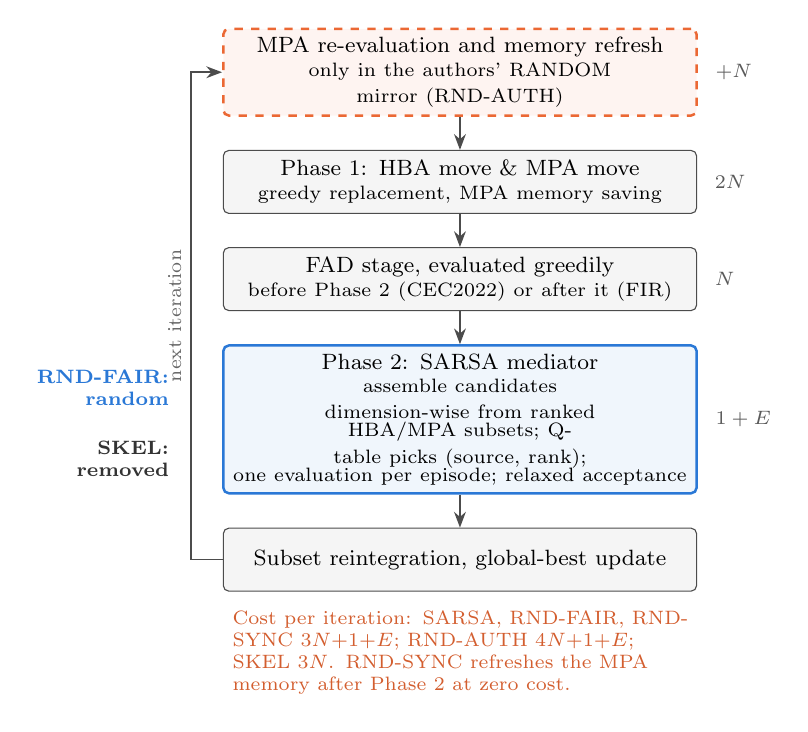
\begin{tikzpicture}[
  font=\footnotesize,
  node distance=4.2mm,
  box/.style={draw=black!70, rounded corners=2pt, fill=black!4, align=center,
              text width=58mm, inner sep=3pt, minimum height=8mm},
  med/.style={box, draw=lblue, line width=0.9pt, fill=lblue!7},
  extra/.style={box, draw=lorange, dashed, line width=0.9pt, fill=lorange!7},
  cost/.style={font=\scriptsize\itshape, text=black!65, anchor=west, align=left},
  tag/.style={font=\scriptsize\bfseries, text=black!80, anchor=east, align=right},
  arr/.style={-{Stealth[length=2mm]}, black!70, line width=0.6pt}]
  \node[extra] (re) {MPA re-evaluation and memory refresh\\[-1pt]
        {\scriptsize only in the authors' \mbox{RANDOM} mirror (RND-AUTH)}};
  \node[box, below=of re] (p1) {Phase 1: HBA move \& MPA move\\[-1pt]{\scriptsize greedy replacement, MPA memory saving}};
  \node[box, below=of p1] (fad) {FAD stage, evaluated greedily\\[-1pt]
        {\scriptsize before Phase 2 (CEC2022) or after it (FIR)}};
  \node[med, below=of fad] (p2) {Phase 2: SARSA mediator\\[-1pt]
        {\scriptsize assemble candidates dimension-wise from ranked}\\[-3pt]
        {\scriptsize HBA/MPA subsets; Q-table picks (source, rank);}\\[-3pt]
        {\scriptsize one evaluation per episode; relaxed acceptance}};
  \node[box, below=of p2] (ri) {Subset reintegration, global-best update};

  \node[cost] at ($(re.east)+(1mm,0)$) {$+N$};
  \node[cost] at ($(p1.east)+(1mm,0)$) {$2N$};
  \node[cost] at ($(fad.east)+(1mm,0)$) {$N$};
  \node[cost] at ($(p2.east)+(1mm,0)$) {$1+E$};

  \draw[arr] (re) -- (p1);
  \draw[arr] (p1) -- (fad);
  \draw[arr] (fad) -- (p2);
  \draw[arr] (p2) -- (ri);
  \draw[arr] (ri.west) -- ++(-4mm,0) |- node[pos=0.25, rotate=90, above, font=\scriptsize, text=black!60]
        {next iteration} (re.west);

  \node[tag, text=lblue] at ($(p2.west)+(-5.5mm,4mm)$) {RND-FAIR:\\random};
  \node[tag] at ($(p2.west)+(-5.5mm,-5mm)$) {SKEL:\\removed};
  \node[font=\scriptsize, text=lorange!90!black, align=left, anchor=north west, text width=58mm]
        at ($(ri.south west)+(0,-1.2mm)$)
        {Cost per iteration: SARSA, RND-FAIR, RND-SYNC $3N{+}1{+}E$; RND-AUTH $4N{+}1{+}E$; SKEL $3N$.
         RND-SYNC refreshes the MPA memory after Phase 2 at zero cost.};
\end{tikzpicture}
}
\caption{One MPHBS iteration with its evaluation cost ($N$ agents per population, $E$ mediator episodes). The dashed block
exists only in the authors' random mirror. The arms of Table~\ref{tab:arms} replace the mediator's policy (RND-FAIR),
remove Phase~2 (SKEL), or refresh the MPA memory after Phase~2 at no cost (RND-SYNC).}
\label{fig:loop}
\end{figure}

%% =====================================================================
\section{Study design}
\label{sec:design}

The design, hypotheses, run counts, statistics and decision rule were fixed in a pre-registration that was frozen and
tagged in the public repository before any campaign run (Section~\ref{sec:availability}). We summarise it here; no
analysis reported as confirmatory deviates from it.

\subsection{Arms}
All arms are implemented on a validated Python port of the authors' code (Section~\ref{sec:validation}) and use the
authors' final configuration of each benchmark (Table~\ref{tab:arms}).
\textbf{SARSA} is MPHBS unchanged.
\textbf{RND-FAIR} draws source and rank uniformly at random for all $K$ candidates and never reads or updates a Q-table;
everything else, including the evaluation cost, is identical to SARSA.
\textbf{RND-SYNC} (CEC2022 only) is RND-FAIR plus the mirror's memory refresh, performed at zero evaluation cost because
all fitness values are known; on FIR it would be identical to RND-FAIR.
\textbf{RND-AUTH} is a faithful port of the authors' mirror, including the extra re-evaluation.
\textbf{SKEL} is the MPHBS loop with Phase~2 removed.
\textbf{MPHB} is the authors' backbone without mediator, whose loop differs from MPHBS's in that its FAD perturbation is
not evaluated in place but replaces the population and is evaluated in the next iteration.
Secondary arms vary the number of episodes ($N_i$), remove proxy screening ($K=1$), make the acceptance greedy, or add the
memory refresh to SARSA (SARSA-SYNC).

% generated by scripts/paper_assets.py from configs/pathA.yaml -- do not edit
\begin{table*}[t]
\centering
\caption{Primary arms. All arms use the authors' final configuration of the domain (B-C1 on CEC2022, A-C1 on FIR)
and the same total budget (200{,}000 FE on CEC2022, 150{,}000 FE on FIR); the number of iterations $T$ follows from
the per-iteration cost. $N=30$; $E=24$ (CEC2022) and $72$ (FIR) mediator episodes per iteration.}
\label{tab:arms}
\small
\begin{tabular}{llcccc}
\toprule
 & & \multicolumn{2}{c}{FE per iteration} & \multicolumn{2}{c}{Iterations $T$} \\
\cmidrule(lr){3-4}\cmidrule(lr){5-6}
Arm & Change relative to MPHBS & CEC2022 & FIR & CEC2022 & FIR \\
\midrule
SARSA & none (reference: MPHBS) & 115 & 163 & 1738 & 919 \\
RND-FAIR & uniform random assembly, no Q-table & 115 & 163 & 1738 & 919 \\
RND-SYNC & RND-FAIR + zero-FE MPA memory refresh & 115 & -- & 1738 & -- \\
RND-AUTH & authors' RANDOM mirror (+N re-evaluations) & 145 & 193 & 1378 & 776 \\
SKEL & no Phase~2 (no mediator) & 90 & 90 & 2221 & 1666 \\
MPHB & authors' backbone without mediator & 90 & 90 & 2221 & 1666 \\
\bottomrule
\end{tabular}
\end{table*}


\subsection{Hypotheses}
Each hypothesis is a paired comparison of two arms (anchor first), tested separately on each benchmark:
\textbf{H1} (learning) SARSA vs RND-FAIR;
\textbf{H2a} (budget of the published mirror) RND-SYNC vs RND-AUTH on CEC2022 and RND-FAIR vs RND-AUTH on FIR, which
differ only in the extra evaluations;
\textbf{H2b} (memory refresh, CEC2022) RND-FAIR vs RND-SYNC;
\textbf{H3} (mediator) SARSA vs SKEL;
\textbf{H4} (loop) SKEL vs MPHB.
H1--H4 are confirmatory. The escape rate on CEC2022 F10 (H5), the number of episodes (H6), the mediator's components (H7)
and the memory refresh in SARSA (H8) are exploratory.

\subsection{Benchmarks, runs and seeds}
CEC2022~\cite{kumar2021cec2022} F1--F12 at $D=20$ with 200{,}000 evaluations (official C code), and the eight FIR
filter-design cases of~\cite{flores2026mphbs} (low-pass, high-pass, band-pass and band-stop, each in an easier and a harder
variant) at $D=31$ with 150{,}000 evaluations. The outcome is the final
error (CEC2022) or objective value (FIR). The H1 pair was run 100 times per instance and every other arm 50 times; F10
was extended to 100 runs for the four H5 arms. Seeds are $\text{seed} = 92\,000\,000 + \text{offset} + 1000\cdot
\text{instance} + \text{run}$, identical across arms, so all comparisons are seed-paired. The H1 run count was chosen so
that a practical-equivalence claim has adequate power (pre-registration, Section~4).

\subsection{Statistics and decision rule}
For each instance we compute a two-sided paired Wilcoxon signed-rank test and the paired win probability
$\hat w=(\text{wins}+0.5\,\text{ties})/n$ of the anchor; values within $10^{-12}$ are ties. $p$-values are Holm-adjusted
within each (hypothesis, benchmark) family~\cite{holm1979,derrac2011tutorial}. The domain-level effect $\bar W$ is the mean
of $\hat w$ over instances, with a 95\% percentile bootstrap interval~\cite{efron1979bootstrap} obtained by resampling runs
within instances. The verdict is applied mechanically in this order: \emph{mixed} if Holm-significant instances favour both
arms; \emph{anchor (comparator) superior} if at least one Holm-significant instance favours it and the interval for
$\bar W$ lies entirely above (below) $0.5$; \emph{practically equivalent} if the interval lies within $[0.44, 0.56]$, the
negligible-effect band of Vargha and Delaney~\cite{vargha2000}, and no instance is significant; otherwise
\emph{inconclusive}. Escape rates (H5) are reported with Wilson intervals~\cite{wilson1927} and compared by an exact
McNemar test~\cite{mcnemar1947}.

\subsection{Execution and validation}
\label{sec:validation}
The campaign ran once on GitHub-hosted Linux runners in the pinned software environment (Python 3.11, NumPy 2.4.6),
after the full test suite had passed there. The port's MPHBS reproduces the authors' evaluation totals exactly and their
published run distributions~\cite{flores2026code}; the one known exception, a lower escape rate on F10, is examined in H5.
Unit tests establish that (i) the variant code with default settings is bit-identical to the validated MPHBS port;
(ii) every arm's evaluation total matches Table~\ref{tab:arms}; (iii) at a fixed number of iterations and on test problems, RND-AUTH produces
trajectories bit-identical to RND-FAIR under the FIR configuration and to RND-SYNC under the CEC2022 configuration, so the re-evaluation itself has no effect
other than its cost; and (iv) removing the writes of the global-best injection does not change any trajectory. All
\res{runs-total} runs completed with the expected evaluation totals, and re-running the analysis on the stored raw results on a
second machine reproduced all verdicts, effect sizes and intervals. RND-AUTH agrees with the authors' published mirror runs on every instance
(two-sided Mann--Whitney, Holm; \res{V3-CEC2022-differ} of \res{V3-CEC2022-n} and \res{V3-FIR-differ} of \res{V3-FIR-n}
instances differ).

%% =====================================================================
\section{Results}
\label{sec:results}

Table~\ref{tab:primary} lists the confirmatory verdicts and Fig.~\ref{fig:instances} the per-instance effects.

% generated by scripts/paper_assets.py -- do not edit
\begin{table*}[t]
\centering
\caption{Confirmatory contrasts (pre-registered H1--H4). Sig.\ (A/C): number of instances significant after Holm in favour of the anchor / comparator. $\bar W$: mean paired win probability of the anchor with 95\% bootstrap CI. Verdicts by the frozen decision rule.}
\label{tab:primary}
\small
\begin{tabular}{llllrcccl}
\toprule
 & Domain & Anchor & Comparator & $n$ & Sig.\ (A/C) & $\bar W$ & 95\% CI & Verdict \\
\midrule
H1 & CEC2022 & SARSA & RND-FAIR & 100 & 0/1 & 0.461 & [0.434, 0.489] & comparator \\
H1 & FIR & SARSA & RND-FAIR & 100 & 0/1 & 0.443 & [0.409, 0.476] & comparator \\
H2a & CEC2022 & RND-SYNC & RND-AUTH & 50 & 0/0 & 0.534 & [0.495, 0.573] & inconclusive \\
H2a & FIR & RND-FAIR & RND-AUTH & 50 & 1/0 & 0.575 & [0.527, 0.623] & anchor \\
H2b & CEC2022 & RND-FAIR & RND-SYNC & 50 & 9/2 & 0.717 & [0.690, 0.743] & mixed \\
H3 & CEC2022 & SARSA & SKEL & 50 & 4/2 & 0.579 & [0.545, 0.613] & mixed \\
H3 & FIR & SARSA & SKEL & 50 & 8/0 & 0.962 & [0.943, 0.980] & anchor \\
H4 & CEC2022 & SKEL & MPHB & 50 & 12/0 & 0.780 & [0.757, 0.802] & anchor \\
H4 & FIR & SKEL & MPHB & 50 & 8/0 & 0.826 & [0.798, 0.853] & anchor \\
\bottomrule
\end{tabular}
\end{table*}


\begin{figure*}[t]
\centering
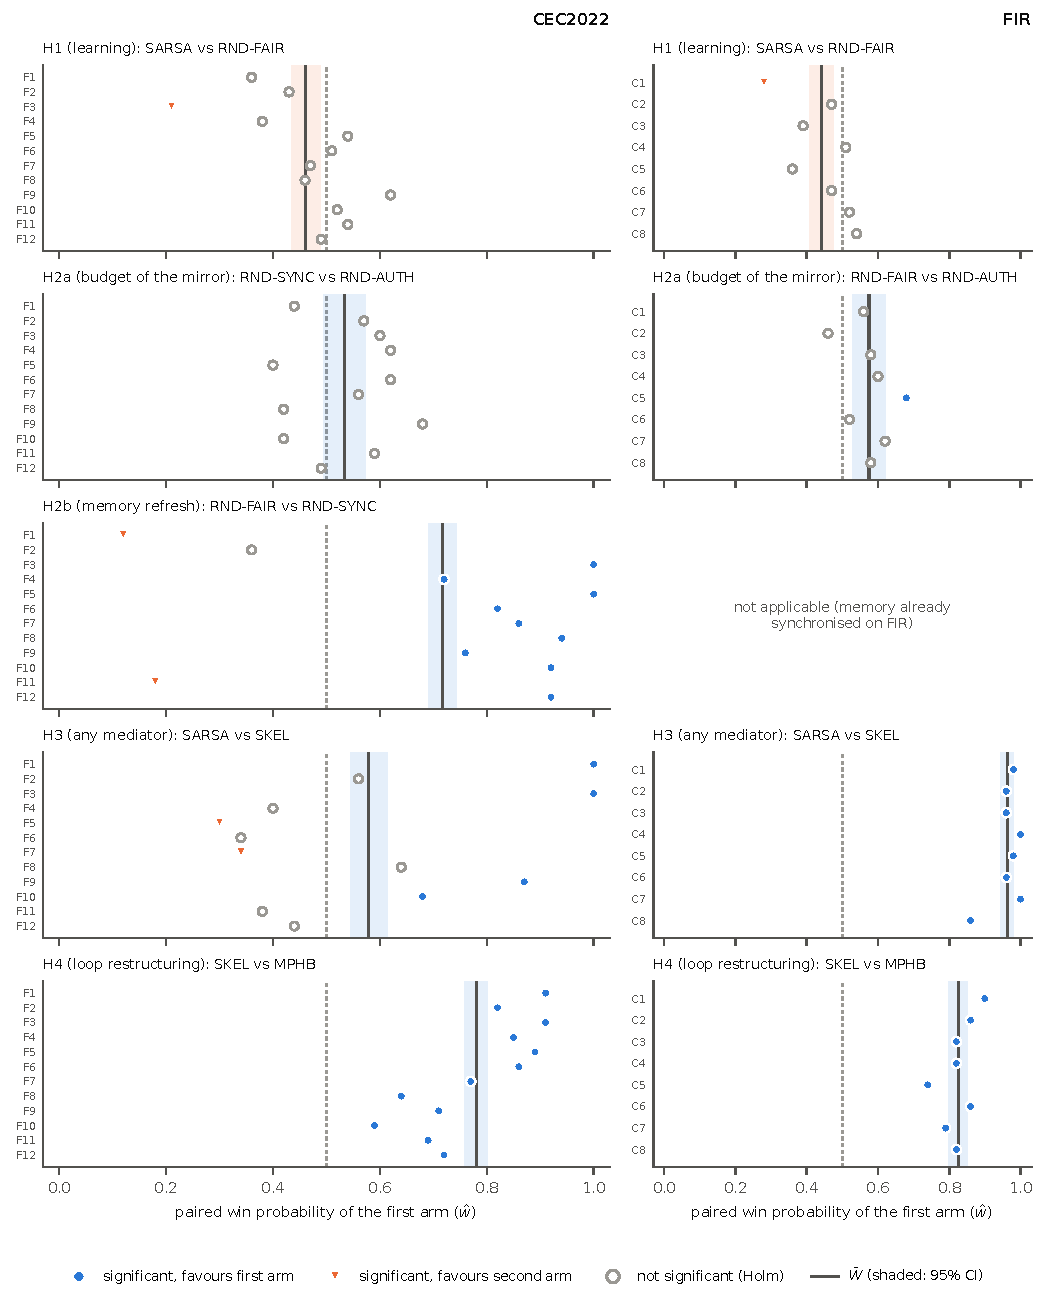
\includegraphics[width=0.92\textwidth]{figures/fig_instances.pdf}
\caption{Per-instance paired win probability $\hat w$ of the first arm for the confirmatory hypotheses
(F: CEC2022 function, C: FIR case). Filled markers are significant after Holm correction; the vertical line and band show
$\bar W$ and its 95\% bootstrap interval; the dotted line marks no difference.}
\label{fig:instances}
\end{figure*}

\subsection{H1: learning}
At equal budget, SARSA does not outperform random assembly on either benchmark. On CEC2022 SARSA's mean paired win
probability is \res{H1-CEC2022-wbar} \res{H1-CEC2022-ci}, and on FIR \res{H1-FIR-wbar} \res{H1-FIR-ci}. Both intervals lie
below $0.5$ and one instance per benchmark is significant in favour of the random mediator (CEC2022 F3, FIR case 1;
Table~\ref{tab:h1}), so the pre-registered verdict is \emph{comparator superior} on both. The effect is small: no
instance favours SARSA, and the median errors of the two arms are close on most instances.

% generated by scripts/paper_assets.py -- do not edit
\begin{table}[t]
\centering
\caption{H1 per instance: SARSA vs RND-FAIR, 100 seed-paired runs each. Medians of the final error;
W/T/L from SARSA's view; $\hat w$ = paired win probability of SARSA; $p$ two-sided Wilcoxon, Holm-adjusted within
domain. $^{\downarrow}$ significant in favour of RND-FAIR.}
\label{tab:h1}
\scriptsize
\setlength{\tabcolsep}{3pt}
\begin{tabular}{llllccc}
\toprule
 & Inst. & SARSA & RND-FAIR & W/T/L & $\hat w$ & $p_\mathrm{Holm}$ \\
\midrule
CEC2022 & F1 & $2.43{\times}10^{-7}$ & $1.59{\times}10^{-7}$ & 36/0/64 & 0.36 & 0.635 \\
CEC2022 & F2 & 44.9 & 49.08 & 43/0/57 & 0.43 & 1 \\
CEC2022 & F3 & $1.63{\times}10^{-5}$ & $4.39{\times}10^{-6}$ & 21/0/79 & 0.21$^{\downarrow}$ & $1.0{\times}10^{-7}$ \\
CEC2022 & F4 & 37.31 & 33.83 & 38/0/62 & 0.38 & 0.180 \\
CEC2022 & F5 & 17.67 & 17.04 & 54/0/46 & 0.54 & 1 \\
CEC2022 & F6 & 20.02 & 17.65 & 51/0/49 & 0.51 & 1 \\
CEC2022 & F7 & 30.1 & 29.92 & 47/0/53 & 0.47 & 1 \\
CEC2022 & F8 & 20.96 & 21.01 & 46/0/54 & 0.46 & 1 \\
CEC2022 & F9 & 180.8 & 180.8 & 58/8/34 & 0.62 & 0.158 \\
CEC2022 & F10 & 100.4 & 100.4 & 52/0/48 & 0.52 & 1 \\
CEC2022 & F11 & 300 & 300 & 54/0/46 & 0.54 & 1 \\
CEC2022 & F12 & 240.1 & 240.8 & 49/0/51 & 0.49 & 1 \\
\midrule
FIR & Case 1 & $5.17{\times}10^{-3}$ & $4.81{\times}10^{-3}$ & 28/0/72 & 0.28$^{\downarrow}$ & $1.3{\times}10^{-4}$ \\
FIR & Case 2 & 0.02158 & 0.02137 & 47/0/53 & 0.47 & 1 \\
FIR & Case 3 & $5.09{\times}10^{-3}$ & $4.82{\times}10^{-3}$ & 39/0/61 & 0.39 & 0.181 \\
FIR & Case 4 & 0.02151 & 0.02124 & 51/0/49 & 0.51 & 1 \\
FIR & Case 5 & $1.74{\times}10^{-3}$ & $1.41{\times}10^{-3}$ & 36/0/64 & 0.36 & 0.335 \\
FIR & Case 6 & $8.34{\times}10^{-3}$ & $6.77{\times}10^{-3}$ & 47/0/53 & 0.47 & 1 \\
FIR & Case 7 & $1.32{\times}10^{-3}$ & $1.60{\times}10^{-3}$ & 52/0/48 & 0.52 & 1 \\
FIR & Case 8 & $3.69{\times}10^{-3}$ & $3.81{\times}10^{-3}$ & 54/0/46 & 0.54 & 1 \\
\bottomrule
\end{tabular}
\end{table}


\subsection{H2: the published mirror}
With the memory refresh held fixed, the extra evaluations of the published mirror do not produce a conclusive difference
on CEC2022 ($\bar W=\res{H2a-CEC2022-wbar}$ \res{H2a-CEC2022-ci}, verdict \emph{inconclusive}). On FIR, where the
re-evaluation affects only the budget, the budget-identical random mediator is better than the published mirror
($\bar W=\res{H2a-FIR-wbar}$ \res{H2a-FIR-ci}, \emph{anchor superior}). The memory refresh, by contrast, has a large effect on
CEC2022 (H2b): random assembly \emph{without} the refresh beats the same mediator with it on
\res{H2b-CEC2022-siga} of 12 functions ($\bar W=\res{H2b-CEC2022-wbar}$ \res{H2b-CEC2022-ci}), for instance on F5 with median
errors of \res{H2b-CEC2022-i5-amed} and \res{H2b-CEC2022-i5-cmed}. Because \res{H2b-CEC2022-sigc} functions (F1, F11) favour
the refresh, the verdict is \emph{mixed}. Together, H2a and H2b explain the published SARSA-versus-mirror difference on
CEC2022 without any contribution of learning: the published mirror carries a handicap that is mostly due to the memory
refresh on CEC2022 and to the reduced budget on FIR.

\subsection{H3 and H4: what does matter}
Removing the mediator altogether is very costly on FIR: SARSA beats SKEL on all eight cases
($\bar W=\res{H3-FIR-wbar}$ \res{H3-FIR-ci}). On CEC2022 the effect is mixed ($\bar W=\res{H3-CEC2022-wbar}$): the mediator
helps on F1, F3, F9 and F10 and hurts on F5 and F7. The exchange of information between the two populations is therefore
useful, but the evidence indicates that its value does not depend on learned choices of source and rank.

The restructured loop is itself a large source of improvement. SKEL, which has no mediator, beats MPHB on every CEC2022
function ($\bar W=\res{H4-CEC2022-wbar}$ \res{H4-CEC2022-ci}) and every FIR case ($\bar W=\res{H4-FIR-wbar}$
\res{H4-FIR-ci}). The two loops differ mainly in whether the FAD perturbation is evaluated with greedy acceptance; this change
therefore accounts for part of the advantage of MPHBS over its backbone that a comparison of MPHBS with MPHB alone would
attribute to the mediator.

\subsection{Exploratory results (H5--H8)}
\textbf{F10 escapes.} SARSA escapes the local basin of F10 in \res{H5-SARSA-esc}/\res{H5-SARSA-n} runs
(Wilson 95\% interval \res{H5-SARSA-ci}) and RND-FAIR in \res{H5-RND-FAIR-esc}/\res{H5-RND-FAIR-n} (\res{H5-RND-FAIR-ci};
exact McNemar $p=\res{H5-mcnemar-p}$); RND-AUTH escapes in \res{H5-RND-AUTH-esc}/\res{H5-RND-AUTH-n} and SKEL in
\res{H5-SKEL-esc}/\res{H5-SKEL-n}. Escaping requires the mediator but not learning. The authors' 17/30 escapes for SARSA are
inconsistent with our 100-seed estimate (binomial $p=\res{H5-binom-p}$); since our port reproduces their other published
distributions, we regard their single F10 sample as unrepresentative but cannot rule out a platform-dependent effect.

\textbf{Mediator components and budget.} Removing proxy screening (H7, $K=1$) or relaxed acceptance leaves performance
practically unchanged or inconclusive (Table~\ref{tab:secondary}). Fewer episodes per iteration are clearly worse on FIR
($N_i=1$ vs $9$: $\bar W=\res{H6-RND-Ni1-vs-default-FIR-wbar}$ \res{H6-RND-Ni1-vs-default-FIR-ci}), whereas no tested $N_i$
shows a consistent advantage of SARSA over random assembly (Table~\ref{tab:secondary}).

\textbf{Memory refresh in SARSA.} Adding the zero-cost refresh to SARSA reproduces the H2b pattern
(H8, $\bar W=\res{H8-CEC2022-wbar}$ \res{H8-CEC2022-ci}): the stale memory of MPHBS is beneficial on most CEC2022 functions.
\pending{diversity diagnostic: population diversity and reversion counts per iteration for SARSA vs SARSA-SYNC, from the
stored traces, to test the explanation below.}

% generated by scripts/paper_assets.py -- do not edit
\begin{table*}[t]
\centering
\caption{Exploratory contrasts (H6--H8), same statistics as Table~\ref{tab:primary}; no claim rests on them.}
\label{tab:secondary}
\small
\begin{tabular}{llllrcccl}
\toprule
 & Domain & Anchor & Comparator & $n$ & Sig.\ (A/C) & $\bar W$ & 95\% CI & Verdict \\
\midrule
H6 policy, $N_i{=}1$ & CEC2022 & SARSA ($N_i{=}1$) & RND ($N_i{=}1$) & 50 & 0/0 & 0.465 & [0.427, 0.504] & inconclusive \\
H6 policy, $N_i{=}1$ & FIR & SARSA ($N_i{=}1$) & RND ($N_i{=}1$) & 50 & 0/1 & 0.470 & [0.422, 0.518] & inconclusive \\
H6 policy, $N_i{=}3$ & CEC2022 & SARSA & RND-FAIR & 50 & 0/1 & 0.435 & [0.396, 0.473] & comparator \\
H6 policy, $N_i{=}3$ & FIR & SARSA ($N_i{=}3$) & RND ($N_i{=}3$) & 50 & 0/0 & 0.435 & [0.387, 0.483] & inconclusive \\
H6 policy, $N_i{=}9$ & CEC2022 & SARSA ($N_i{=}9$) & RND ($N_i{=}9$) & 50 & 1/1 & 0.490 & [0.450, 0.528] & mixed \\
H6 policy, $N_i{=}9$ & FIR & SARSA & RND-FAIR & 50 & 0/0 & 0.450 & [0.403, 0.498] & inconclusive \\
H6 $N_i{=}1$ vs default & CEC2022 & RND ($N_i{=}1$) & RND-FAIR & 50 & 2/2 & 0.477 & [0.441, 0.515] & mixed \\
H6 $N_i{=}1$ vs default & FIR & RND ($N_i{=}1$) & RND-FAIR & 50 & 0/4 & 0.345 & [0.300, 0.390] & comparator \\
H6 other $N_i$ vs default & CEC2022 & RND ($N_i{=}9$) & RND-FAIR & 50 & 1/3 & 0.448 & [0.411, 0.486] & mixed \\
H6 other $N_i$ vs default & FIR & RND ($N_i{=}3$) & RND-FAIR & 50 & 0/1 & 0.495 & [0.448, 0.543] & inconclusive \\
H7 $K{=}1$ & CEC2022 & RND-K1 & RND-FAIR & 50 & 0/1 & 0.486 & [0.448, 0.524] & inconclusive \\
H7 $K{=}1$ & FIR & RND-K1 & RND-FAIR & 50 & 0/0 & 0.512 & [0.465, 0.560] & equivalent \\
H7 greedy accept. & CEC2022 & RND-GreedyAcc & RND-FAIR & 50 & 0/0 & 0.507 & [0.468, 0.547] & equivalent \\
H7 greedy accept. & FIR & RND-GreedyAcc & RND-FAIR & 50 & 0/1 & 0.483 & [0.435, 0.530] & inconclusive \\
H8 & CEC2022 & SARSA-SYNC & SARSA & 50 & 2/9 & 0.277 & [0.252, 0.303] & mixed \\
\bottomrule
\end{tabular}
\end{table*}


%% =====================================================================
\section{Discussion}
\label{sec:discussion}

\subsection{What drives MPHBS}
Three components carry the performance of MPHBS on these benchmarks: exchanging information between the two populations
at all, the amount of exchange per iteration, and the evaluated FAD stage of its loop. The SARSA controller is not among
them: random choices of source and rank are at least as good. A plausible reason is the reward signal. It is the sign of
the improvement of a single assembled vector over the current one, which says little about which (source, rank) pair
helped, while the proxy screening and the acceptance rule already bias the search towards good candidates.

The memory finding suggests a mechanism. When MPHBS leaves the memory stale, MPA agents that move to worse positions
revert to where they were before the mediator rather than to the post-mediator population, whose subset rows the mediator
has filled with copies of vectors close to the incumbent. The stale memory may therefore preserve diversity. This
explanation is exploratory and is tested by the pending diagnostic above.

\subsection{Requirements for ablation controls of learned components}
\begin{enumerate}
\item \textbf{Match the cost per iteration, not only the total budget.} When runs are cut by a total evaluation budget,
  any extra evaluation per iteration silently reduces the number of iterations of the control.
\item \textbf{Match every state update.} A control should be derived from the learned variant by removing the learning,
  not written as a separate program; side effects such as memory or archive updates must be identical.
\item \textbf{Verify equivalence mechanically.} With fixed seeds, the control with learning ``switched off'' in the same
  code path, and unit tests showing bit-identical trajectories where no difference is intended, rule out accidental
  differences.
\item \textbf{Separate the learned component from the mechanism it controls.} A no-mediator arm and a random-policy arm
  answer different questions (H3 vs H1); both are needed.
\item \textbf{Fix the analysis in advance.} Pre-registered hypotheses, run counts and decision rules prevent post hoc
  selection of the favourable comparison~\cite{nosek2018preregistration,lopezibanez2021reproducibility,bartzbeielstein2020benchmarking}.
\end{enumerate}

\subsection{Threats to validity}
\textbf{Scope.} We study one hybrid, two benchmark sets at one dimension each, and the authors' final configurations.
Those configurations were selected with SARSA on the same benchmarks, which favours SARSA and makes H1 conservative.
\pending{exploratory BBOB extension~\cite{hansen2021coco} to test whether H1 generalises.}
\textbf{Port.} Our results use a Python port; agreement with the authors' MATLAB runs is distributional because random
streams differ. The port reproduces the authors' totals and run distributions, and RND-AUTH reproduces their mirror on
all instances.
\textbf{Effect sizes.} The H1 effect is small; we claim the absence of a benefit of learning, not a large benefit of random
choice.
\textbf{Exploratory parts.} H5--H8 and the memory mechanism are exploratory and should be confirmed independently.

%% =====================================================================
\section{Conclusion}
The learned controller of MPHBS does not improve on random choices at equal budget on CEC2022 or FIR; the published
evidence for it rests on a control that is handicapped by its evaluation budget and, on CEC2022, by a memory update.
MPHBS's advantage comes from exchanging information between its populations and from its restructured loop. More
generally, ablations of learned components in metaheuristics should match the per-iteration cost and every state update
of the learned variant, and should be verified mechanically and fixed in advance.

\section*{Data and code availability}
\label{sec:availability}
Code, the frozen pre-registration (tag \texttt{pathA-prereg-frozen}), all \res{runs-total} raw runs, the analysis and
the scripts that generate every number, table and figure in this paper are available at
\url{https://github.com/abinaya-g/la-kaie} (campaign commit \texttt{\res{commit}}). \pending{archive a release on Zenodo and
cite its DOI.}

\section*{CRediT authorship contribution statement}
\pending{CRediT roles.}

\section*{Declaration of competing interest}
\pending{declaration.}

\section*{Acknowledgements}
We thank the authors of MPHBS for publishing their code and per-run results, without which this study would not have
been possible. \pending{funding; whether the MPHBS authors were contacted before submission.}

\bibliographystyle{elsarticle-num}
\bibliography{refs}

\end{document}
